\documentclass[a4paper,11pt,UTF8]{article}
\usepackage{ctex}
\usepackage{amsmath,amsthm,amssymb,amsfonts}
\usepackage{amsmath}
\usepackage[a4paper]{geometry}
\usepackage{graphicx}
\usepackage{microtype}
\usepackage{siunitx}
\usepackage{booktabs}
\usepackage[colorlinks=false, pdfborder={0 0 0}]{hyperref}
\usepackage{cleveref}
\usepackage{esint} 
\usepackage{graphicx}
\usepackage{ragged2e}
\usepackage{pifont}
\usepackage{extarrows}
\usepackage{mathptmx}
\usepackage{float}
\usepackage{caption}
\usepackage{multirow}
\usepackage{subfigure}
\usepackage{titlesec}
\usepackage{makecell}
\usepackage{tabularx}
\usepackage{graphicx}

\numberwithin{equation}{subsection}

\titleformat{\section}{\Large\bfseries}{\thesection}{1em}{}
\titleformat{\subsection}{\large\bfseries}{\thesubsection}{1em}{}
\titleformat{\subsubsection}{\normalsize\bfseries}{\thesubsubsection}{1em}{}
\begin{document}
\begin{titlepage}
	\begin{center}
		\vspace*{1cm}
		\textbf{\LARGE 实验报告:共源放大电路设计、仿真与实现}
		\vspace{0.5cm}
		
		\Large 谢悦晋\quad 提高2201班\quad U20221033
		\vspace{1cm}
		\begin{figure}[H]
			\centering
			\subfigure{
				
\includegraphics[scale=1]{hust}
			}
			\subfigure{
				
\includegraphics[scale=1]{eic}
			}
			\caption*{}
		\end{figure}
		\vfill
		\vspace{0.8cm}
		华中科技大学 \\
		电子信息与通信学院 \\
		Oct 31st, 2023
	\end{center}
\end{titlepage}
\tableofcontents\newpage
\section{实验名称}
共源放大电路设计、仿真与实现
\section{实验目的}
\begin{itemize}
	\item 学习共源放大电路工作原理
	\item 掌握金属-氧化物-半导体场效应管的主要性能参数及其测试方法
	\item 掌握共源放大电路参数调整方法
	\item 掌握共源放大电路的基本原理与参数测量方法
	\item 掌握MOSFET共源极放大电路的安装与测试 技术
	\item 掌握Multisim软件的使用,实现共源放大电路的仿真实现
\end{itemize}
\section{实验元器件}
\begin{table}[h]
	\centering
	\begin{tabular}{|c|c|c|}
		\hline
		名称 & 型号/参数 & 数量\\
		\hline
		场效应管 & 2N7000 & 1\\
		\hline
		\multirow{3}{*}{电容} & 4.7μF & 1 \\
		\cline{2-3}
		 & 47μF & 1\\
		\cline{2-3}
		 & 1μF & 1\\
		\hline
		电位器 & 500kΩ & 1\\
		\hline
		\multirow{4}{*}{电阻} & 100kΩ & 2 \\
		\cline{2-3}
		 & 5.1kΩ & 1\\
		\cline{2-3}
		 & 51kΩ & 1\\
		\cline{2-3}
 		 & 1kΩ & 1\\
		\hline 		
	\end{tabular}
\end{table}
\section{实验任务}
主要为以下三个实验任务:MOSFET输出特性曲线仿真、MOSFET转移特性曲线仿真、MOSFET共源放大电路安装、调试及测试
\subsection{MOSFET输出特性曲线仿真}
使用 OrCAD/Spice 分析绘制 MOSFET (2N7000) 的共源极输出特性曲线。实验步骤与要求如下:

(1)建立新项目,绘出电路图。

首先新建一个工程项目,然后放置元器件(M2N7000、Vdc、0 (GRD)等)、连线,画出如图 3.3.5 所示的电路,并在 MOSFET 的漏极放置电流测试探针

\begin{minipage}[t]{0.6\textwidth}
	(2)设置仿真简表。
	
	\ding{172} 新建仿真简表 (New Simulation Profile), 设置直流扫描分析(DC Sweep) 的主扫描(Primary Sweep), 扫描变量为VDD, 采用线性扫描,由 OV 开始至 8V 结束,步进为  0.01V。
	
	\ding{173} 设置直流扫描分析(DC Sweep)中的二级扫描(Secondray Sweep), 扫描变量为 VGG, 采用线性扫描,由 1.7V 开始至 2.05V 结束,步进为 0.05V。
\end{minipage}
\begin{minipage}[t]{0.4\textwidth}
	\begin{figure}[H]
		\centering
		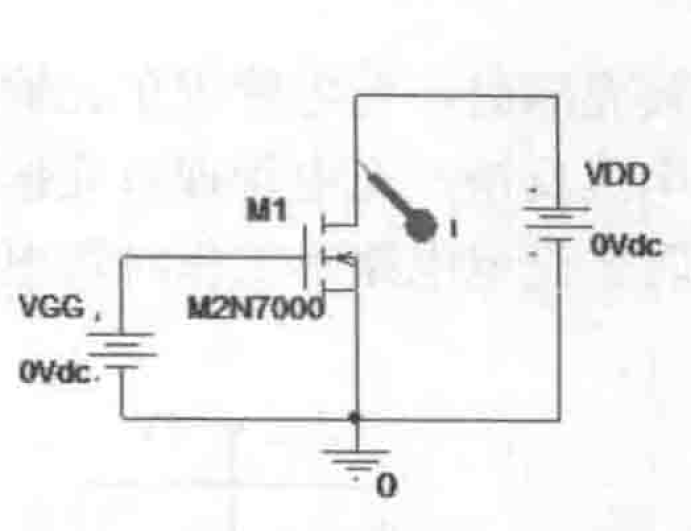
\includegraphics[width=0.75\textwidth]{2.1}
		\caption{特性曲线仿真电路}
	\end{figure}
\end{minipage}


(3)保存文档、执行仿真(Run)。运行后自动打开结果显示窗,显示输出特性曲线($i_\mathrm{D}$ $v_\mathrm{DS}$)。多根曲线对应$v_\mathrm{GS}$ 的间隔为 0.05V。

(4) 将仿真结果反映至实验报告中。

\ding{172} 选中仿真电路图,复制粘贴到实验报告文档中。

\ding{173} 在结果显示窗中,选择 Window\textbackslash Copy to Clipboard...将曲线复制到剪贴板,期间最好选择“change all colors to black”将所有曲线都变为黑色。然后粘贴至实验报告文档。
\subsection{MOSFET转移特性曲线仿真}
使用 OrCAD/Spice 分析绘制 MOSFET (2N7000) 的共源极转移特性曲线。实验步骤与要求如下:

(1)修改电路参数,将$v_\mathrm{op}$电压改为 8V。

(2)设置仿真简表。新建仿真简表(New Simulation Profile), 设置直流扫描分析(DC Sweep)
的主扫描 (Primary Sweep), 扫描变量为 V$_{GG}$, 采用线性扫描,由 OV 开始至 4V 结束,步进为0.01V。

(3)保存文档、执行仿真 (Run)。运行后自动打开结果显示窗,显示转移特性曲线 $(i_\mathrm{D}-v_{\mathrm{GS}})$.

(4) 将仿真结果复制粘贴到实验报告文档中。

\subsection{MOSFET共源放大电路安装、调试及测试}
\begin{figure}[H]
	\centering
	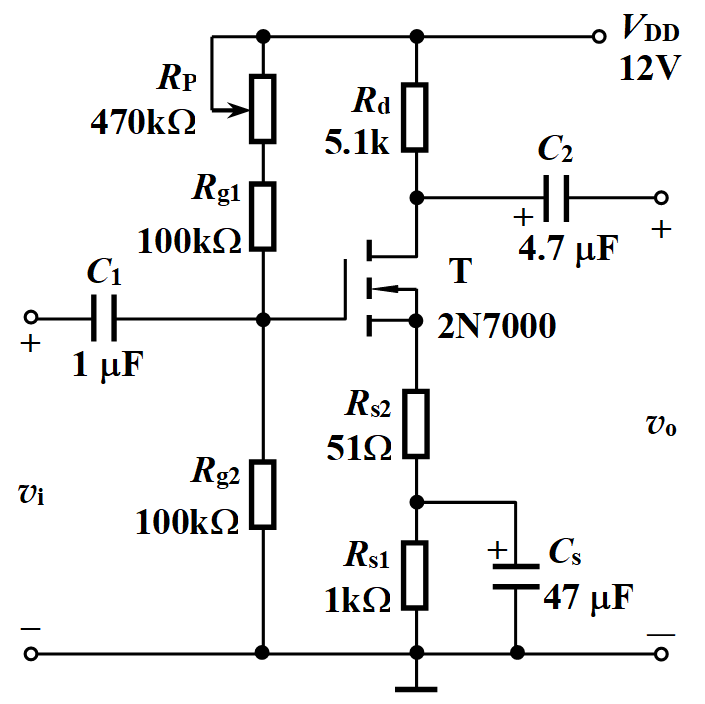
\includegraphics[width=0.6\textwidth]{2.2}
	\caption{共源极放大电路}
\end{figure}

实验步骤与要求如下:

(1)测试电路的静态工作点。 

\ding{172} 按照图3.3.6在面包板上组装电路,$\nu_\mathrm{DD}$的 12V 取自直流稳压电源。安装电阻前先用万用表测试电阻值,填入表 3.3.2 相应栏中。检查无误后接通电源。用数字万用表的直流电压挡测量电路的 $V_\mathrm{G}$ (栅极对地电压)、$V_\mathrm{S}$(源极对地电压)和 $V_\mathrm{D}$(漏极对地电压), 计算静态工作点$Q(I_DQ$、$V_\mathrm{GSQ}$、$V_\mathrm{DSQ}$)。将结果填入表 3.3.2 相应栏中。

\ding{173}关闭电源,将 $R_\mathrm{gl}$ 改为 100k, 检查无误后接通电源,再次测量 $V_\mathrm{G}$、$V_\mathrm{s}$ 和 $V_\mathrm{D}$, 计算静态工作点$\varrho$($I_\mathrm{bQ},V_\mathrm{GSQ},V_\mathrm{DSQ})$。将结果填入表 3.3.2 相应栏中。

\ding{174} 关闭电源,将 $R_\mathrm{gl}$ 恢复为 240k, 而将 $R_{\mathrm{g2}}$ 改为 33k, 检查无误后接通电源,测量 $V_{\mathrm{G}}$、 $V_\mathrm{s}$和$V_\mathrm{D}$, 计算静态工作点$Q$($I_\mathrm{DQ}$、$V_\mathrm{GSQ}$、$V_\mathrm{DSQ}$)。完成表 3.3.2 的内容。
\begin{table}[h]
	\centering
	\resizebox{\linewidth}{!}{\begin{tabular}{|c|c|c|c|c|c|c|c|}
		\hline
		\multirow{2}{*}{} & \multicolumn{3}{c|}{实测值} & \multicolumn{3}{c|}{计算值} & \multirow{2}{*}{\shortstack{MOSFET处于\\哪个工作区}}\\
		\cline{2-7}
		& \small$V_{G}$/V & \small$V_{S}$/V & \small$V_{D}$/V & \small{$I_{DQ}=V_S/R_S$/mA}& \small$V_{GSQ}=(V_G-V_S)$/V & \small$V_{DSQ}=(V_D-V_S)$/V & \\
		\hline
		\small\makecell[l]{$R_{g1}=240k$\\$R_{g2}=100k$} &&&&&&&\\	
		\hline
		\small\makecell[l]{$R_{g1}=100k$\\$R_{g2}=100k$} &&&&&&&\\	
		\hline
		\small\makecell[l]{$R_{g1}=240k$\\$R_{g2}=33k$} &&&&&&&\\
		\hline
		实测电阻值 &\multicolumn{7}{c|}{$R_{g1}=\qquad$,$R_{g2}=\qquad$,$R_{d}=\qquad$,$R_{s}=\qquad$}\\
		\hline				
	\end{tabular}
}
\caption{静态工作点}
\end{table}
(2)测试放大电路的输入、输出波形和通带电压增益。参考上节的图 3.2.7, 搭建放大电路实验测试平台。关闭电源,将电阻参数恢复为
$R_{g1}=240k$, $R_{g2}$=100k, 检查无误后接通电源。调整信号源,使其输出峰-峰值为 30mV、频率为1kHz 的正弦波,作为放大电路的 $v_\mathrm{i}$。分别用示波器的两个通道同时测试 $v_\mathrm{i}$ 和 $v_\mathrm{o}$, 在实验报告上定量画出$v_\mathrm{i}$和$v_\mathrm{o}$的波形(时间轴上下对齐), 分别测试负载开路和 $R_\mathrm{L}=5$.1k$\Omega$两种情况下的 $v_{7}$ 和$v_{0}$,完成表 3.3.3。

(3)测试放大电路的输入电阻。采用在输入回路串入已知电阻的方法测量输入电阻。由于 MOSFET 放大电路的输入电阻
较大,所以当测量仪器的输入电阻不够大时,采用如图 3.2.8 所示的方法可能存在较大误差, 改用如图 3.3.7 所示的测量输出电压的方法更好。$R$ 取值尽量与 $R_i$ 接近(此处可取 R=51k$\Omega$)。信号源仍旧输出峰-峰值 30mV、1kHz 正弦波,用示波器的一个通道始终监视 $v_\mathrm{i}$ 波形,用另个通道先后测量开关 S 闭合和断开时对应的输出电压 $\upsilon_\mathrm{ol}$ 和 $\upsilon_\mathrm{o2}$, 则输入电阻为
\begin{align}R_{\mathrm{i}}=\frac{v_{\mathrm{o}2}}{v_{\mathrm{ol}}-v_{\mathrm{o}2}}\cdot R\end{align}

测量过程要保证 $v_{\mathrm{o}}$不出现失真现象
\begin{figure}[H]
	\begin{minipage}[h]{0.6\textwidth}
		\centering
		\captionsetup{labelsep=space, textformat=simple, format=plain} 
		\renewcommand{\figurename}{表}  
		\resizebox{\linewidth}{!}{\begin{tabular}{|c|c|c|c|c|c|}
				\hline
				\shortstack{负载\\情况} & \shortstack{$v_i$峰-峰\\值$V_{ipp}$/mV} & \shortstack{$v_o$峰-峰值\\$V_{opp}$/mV} & \shortstack{$|A_v|=$\\$V_{opp}/V_{ipp}$}	& \shortstack{$|A_v|$的\\理论值} & \shortstack{相对\\误差}\\
				\hline
				负载开路 & 30 &&&&\\
				\hline
				$R_L=5.1\mathrm{k\Omega}$ & 30 &&&&\\
				\hline		
			\end{tabular}
		}
		\caption{:电压增益($f\mathrm{=}\mathrm{1kHz}$)}
	\end{minipage}
	\begin{minipage}[h]{0.4\textwidth}
		\centering
		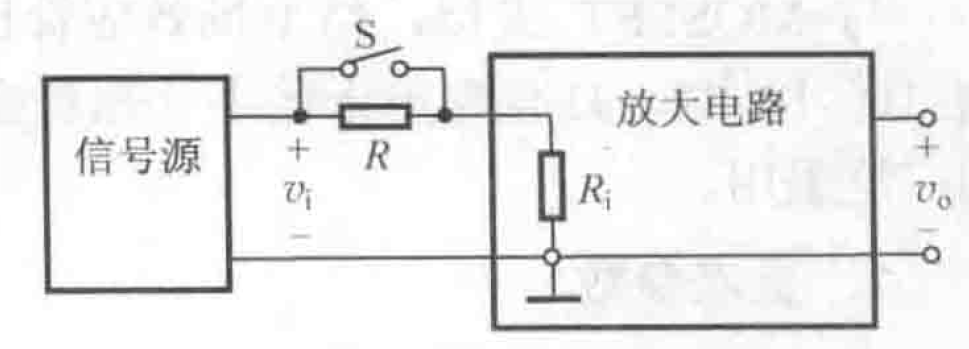
\includegraphics[width=\textwidth]{2.3}
		\caption{高输入电阻测试局部示意图}
	\end{minipage}
\end{figure}

(4)测试放大电路的输出电阻。

采用改委负载的方法测试输出电阻。分别测试负载开路输出电压 $v_o^{\prime}$ 和接入已知负载$R_L$时的输出电压 $v_\mathrm{o}$,测量过程同样要保证 $v_\mathrm{o}$ 不出现失真现象。实际上在表 3.3.3 中已得到 $v_\mathrm{o}^{\prime}$ 和$v_0$, 则输出电阻为
\begin{align}
	R_\mathrm{o}=\frac{v_\mathrm{o}^{\prime}-v_\mathrm{o}}{v_\mathrm{o}^{\prime}}\times R_\mathrm{L}
\end{align}

$R_{\mathrm{L}}$越接近 $R_{o}$ 误差越小。

(5)测试放大电路的通频带。在图3.3.6中,输入$v_\mathrm{i}$ 为峰-峰值 30mV、1kHz 的正弦波,用示波器的一个通道始终监视输入波形的峰-峰值,用另一个通道测出输出波形的峰-峰值。保持输入波形峰-峰值不变,调节信号源的频率,逐渐提高信号的频率,观测输出波形的幅值变化,并相应适时调节示波器水平轴的扫描速率,保证始终能清晰观测到正常的正弦波。持续提高信号频率,直到输出波形峰峰值降为 1kHz 时的 0.707 倍,此时信号的频率即为上限频率 $f_\mathrm{H}$, 记录该频率; 类似地,逐渐降低信号频率,直到输出波形峰-峰值降为 1kHz 时的 0.707 倍,此时的频率即为下限频率 $f_\mathrm{L}$, 记录该频率,完成表 3.3.4。要特别注意,测试过程必须时刻监视输入波形峰-峰值,若有变化,需调整信号源的输出幅值,保持$v_\mathrm{i}$的峰-峰值始终为 30mV。

通频带(带宽)为: 
\begin{align}\mathrm{BW}=f_{\mathrm{H}}-f_{\mathrm{L}}\end{align}
\begin{table}[H]
	\centering
	\begin{tabular}{|c|c|c|c|}
		\hline
		\multirow{2}{*}{信号频率$f$} & $f_L$ & - & $f_H$\\
		\cline{2-4}
		&&1kHz&\\	
		\hline
		\shortstack{输出波形\\峰-峰值$V_{opp}$}&&&\\
		\hline
		$|A_v|$&&&\\
		\hline	
	\end{tabular}
	\caption{通频带($V_{\mathrm{ipp}}=30$mV)}
\end{table}
\section{实验原理}
\subsection{MOSFET共源放大电路安装、调试及测试}
\begin{minipage}[t]{0.6\textwidth}
	图 3.3.6 为 N 沟道增强型 MOSFET 共源极放大电路,其静态工作点可由式(4.3.1) 估算
	\begin{subequations}\begin{align}
			V_{\mathrm{GSQ}}=\frac{R_{\mathrm{g2}}}{R_{\mathrm{g1}}+R_{\mathrm{g2}}}\times V_{\mathrm{DD}}-I_{\mathrm{DQ}}R_{\mathrm{s}}  \\
			I_{\mathrm{DQ}}=K_{\mathrm{n}}\left(V_{\mathrm{GS}}-V_{\mathrm{TN}}\right)^{2} \\
			V_{\mathrm{DSQ}}=V_{\mathrm{DD}}-I_{\mathrm{DQ}}(R_{\mathrm{d}}+R_{\mathrm{s}}) 
	\end{align}\end{subequations}
	动态性能指标可由式(4.1) 估算
	\begin{subequations}\begin{align}
			A_\mathrm{v}=-g_\mathrm{m}R_\mathrm{d}\\
			R_{\mathrm{i}}=R_{\mathrm{g1}}//R_{\mathrm{g2}}\\
			R_{\mathrm{o}}=R_{\mathrm{d}}
	\end{align}\end{subequations}
\end{minipage}
\begin{minipage}[t]{0.4\textwidth}
	\begin{figure}[H]
		\centering
		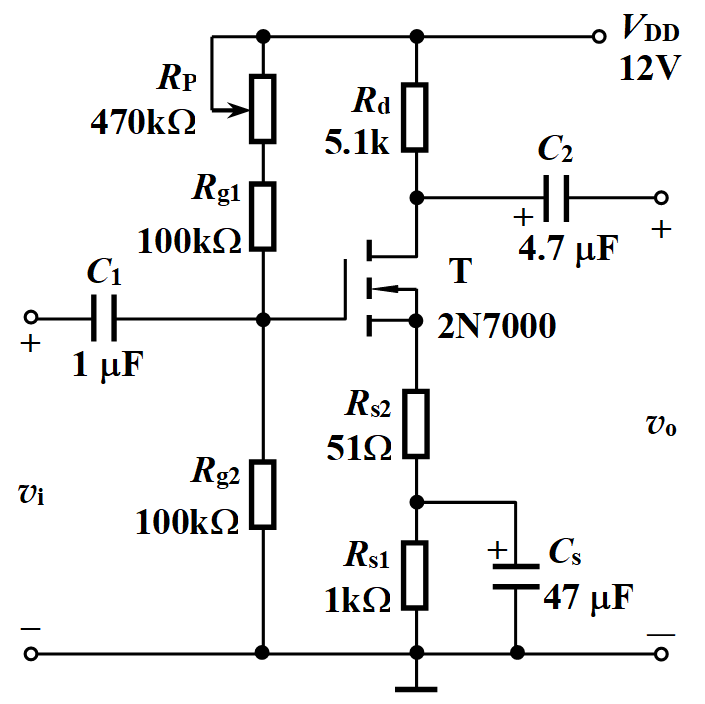
\includegraphics[width=\textwidth]{2.2}
		\caption{共源极放大电路}
	\end{figure}
\end{minipage}

数据手册通常会给出$\nu_\mathrm{TN}$和某工作点下的$g_\mathrm{m}$。由表 3.3.1 看出,对于 MOS 管 2N7000,$I_{\mathrm{D} }= 200$mA 时,$g_m^{\prime}= 100$mS, 可得 $K_n= ( g_m^{\prime}/2) ^2/I_{\mathrm{D} }= 12.5$mA$/V^2$ 式(3.3.4a)中的$g_\mathrm{m}$是图 3.3.6 电路静态工作点下 MOS 管的互导,同样可得
\begin{align}
	g_m&=g_m'\sqrt{I_{\mathrm{DQ}}/I_{\mathrm{D}}}\\
	g_{\mathrm{m}}&=10\sqrt{I_{\mathrm{DQ}}/2}\mathrm{mS}
\end{align}

由数据表可知$V_{\mathrm{TN}}$在0.8-3V之间,这里取 $V_{\mathrm{TN}}=1.75\mathrm{V}$
\subsection{Multisim的使用和学习}
\subsubsection{Multisim介绍}
\noindent Multisim系列软件的组成:
\begin{itemize}
	\item Multisim: 电路仿真设计模块
	\item Ultiboard: PCB设计软件
\end{itemize}

两个部分相互独立,可以分别使用. Multisim系列软件能完成从电路的仿真设计到电路板图生成的全过程。

\noindent 优势:
\begin{itemize}
	\item 操作界面直观易用
	\item 大量元器件库
	\item 虚拟仪器表种仪类齐全,
	\item 分析方法完备
	\item 可调用LabVIEW虚拟仪器(自定义)
	\item 强大的Help 功能,包括软件本身的操作说明、各种元器件功能说明。
\end{itemize}

Multisim经历了多个版本的升级,9版本之后增加了单片机和LabVIEW虚拟仪器的仿真和应用:
\begin{itemize}
	\item 电路分析
	\item 模拟电子电路
	\item 数字电子电路
	\item 模数混合电路
	\item 射频电路
	\item DSP/FPGA/CPLD
	\item 电力电子电路
	\item PLC控制电路
	\item 单片机电路
\end{itemize}

Multisim操作界面:
\begin{figure}[H]
	\centering
	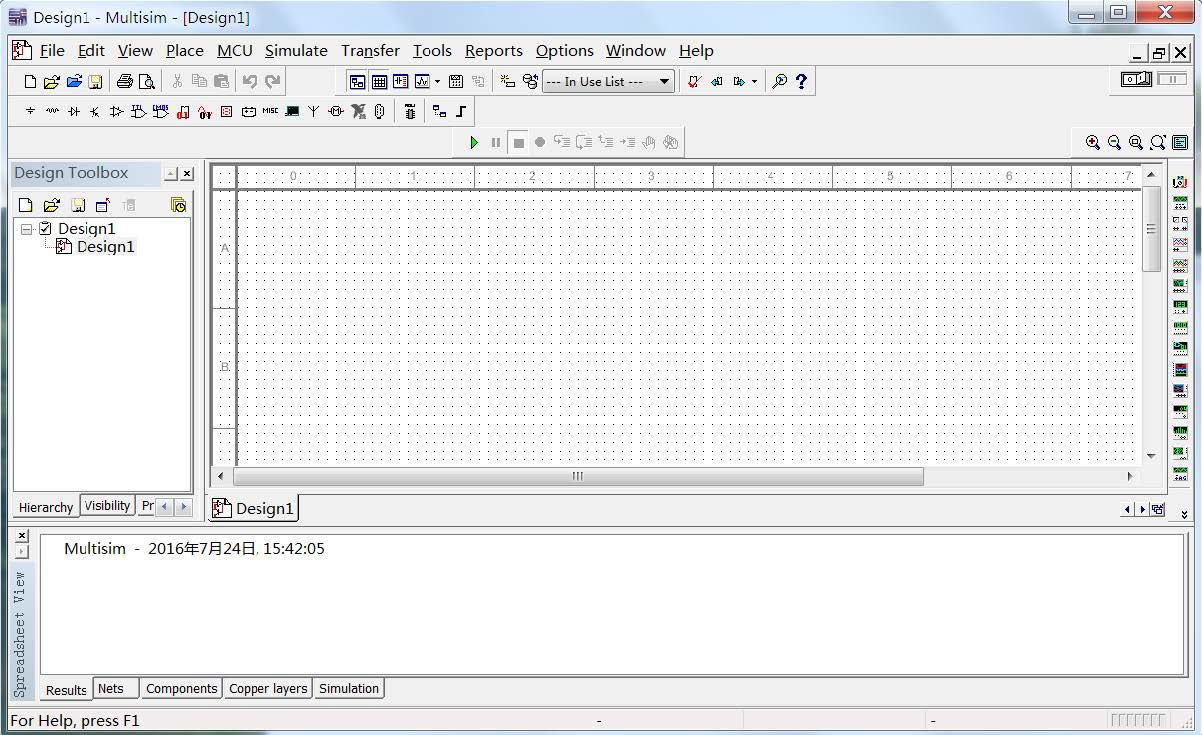
\includegraphics[width=1\textwidth]{MULTISIM}	
\end{figure}

\begin{figure}[H]
	\centering
	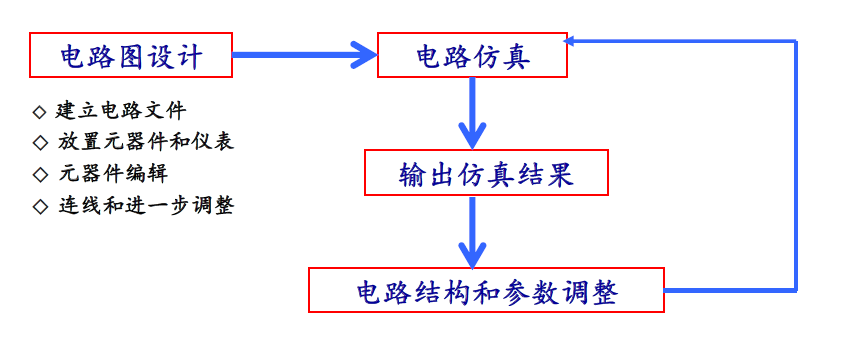
\includegraphics[width=0.7\textwidth]{step}	
\end{figure}
\subsubsection{Multisim 电路图的绘制}
放置元器件(图中红方格内即为常用元器件,点击选中,产生元器件放置即可):
\begin{figure}[H]
	\centering
	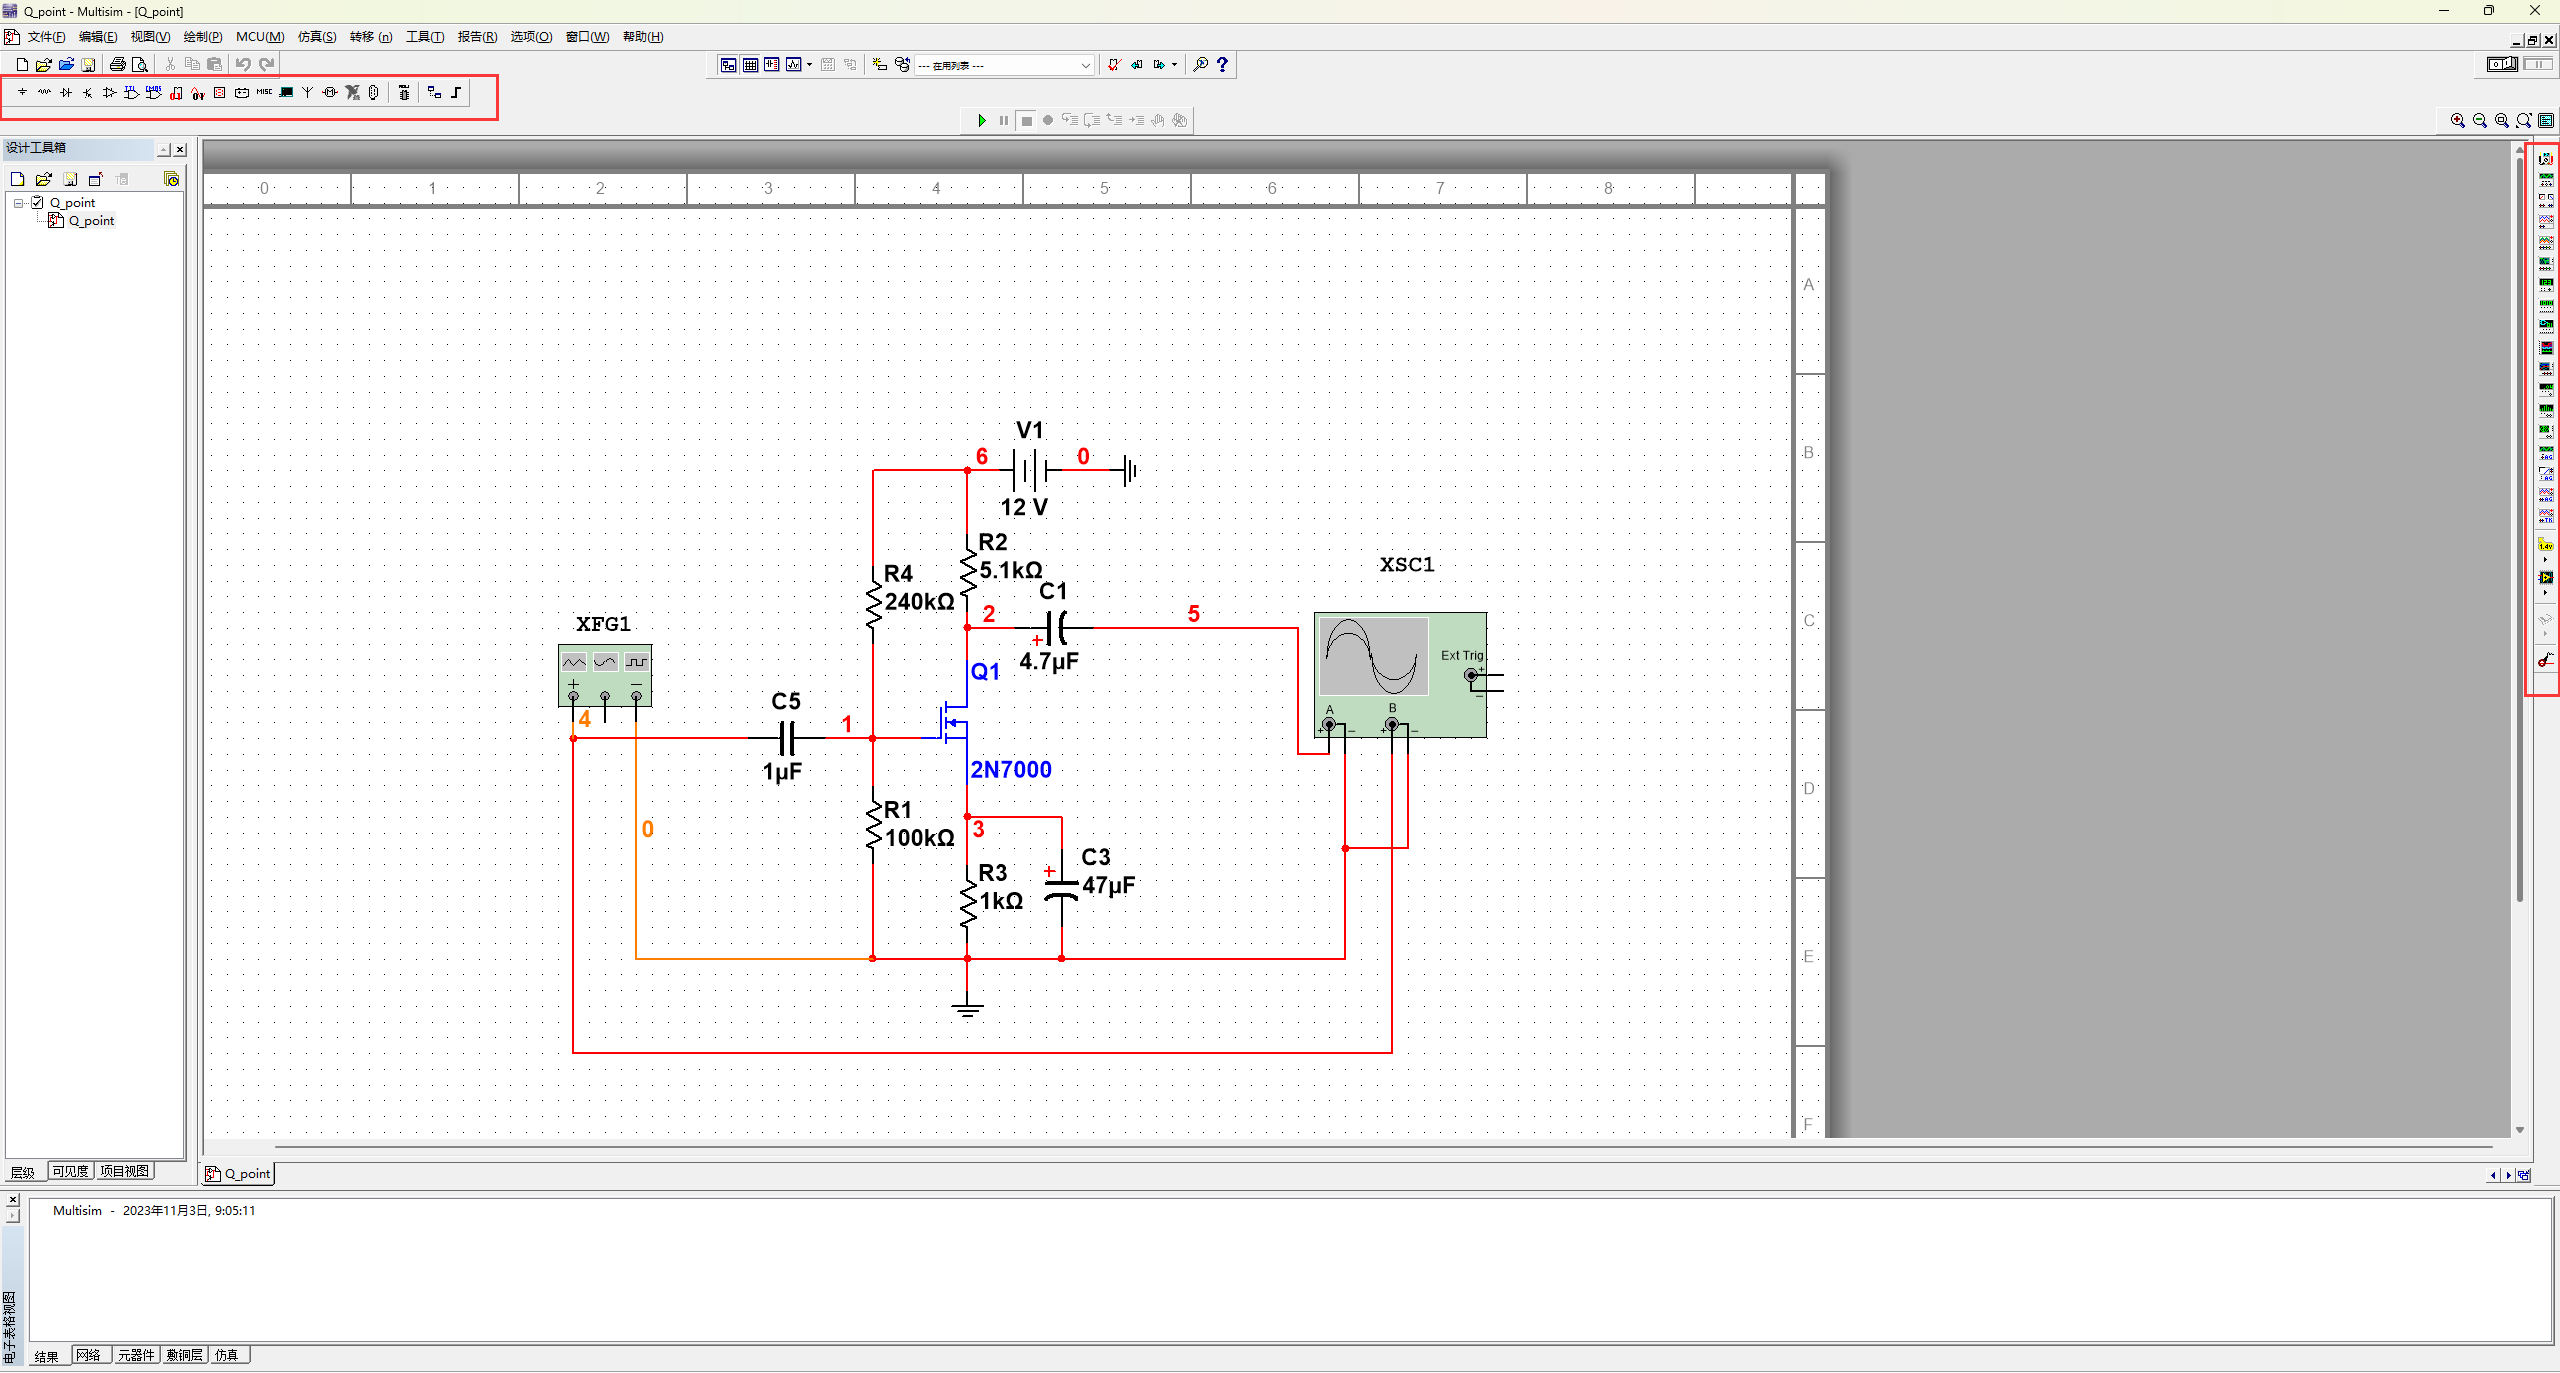
\includegraphics[width=1\textwidth]{5.2.2_1}	
\end{figure}

双击电路工作区中元器件,弹出属性对话框提供元器件参数的修改和设置。
元器件属性对话框具有多种选项可供设置,一般包括Label(标识)、Display (显示)、Value (数值)和 Fault (故障)等几个选项卡的内容。
\begin{figure}[H]
	\centering
	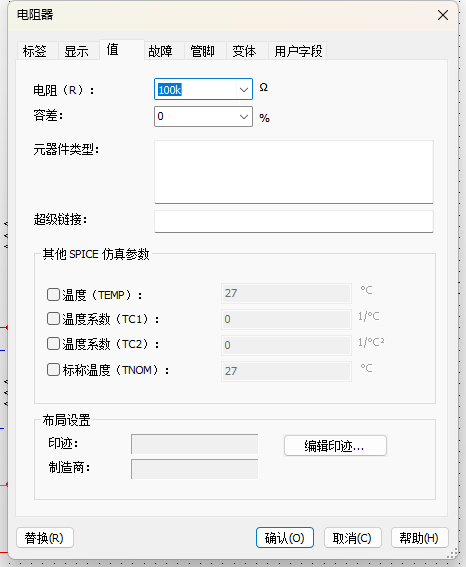
\includegraphics[width=0.4\textwidth]{5.2.2_2}	
\end{figure}

画电路连线:

以连接 12V 电源负极和地之间的导线为例说明自动连线的方法。将鼠标
指向 12V 电源的端点时会出现十字光标,单击鼠标左键,移动十字光标,拖出一根导线,将十字光标指向地的连接端点并单击鼠标左键,即完成了 12V 电源和地之间的导线连接:
\begin{figure}[H]
	\centering
	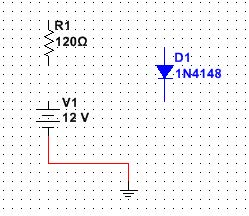
\includegraphics[width=0.3\textwidth]{5.2.2_3}	
\end{figure}
\subsubsection{Multisim 电路仿真分析 }
Multisim12.0提供了多种仿真分析方法,主要包含:直流工作点分析(DC Operation Point Analysis), 交流分析(AC Analysis), 单频交流分析(Single Frequency AC Analysis), 瞬态分析(Transient Analysis), 傅立叶分析(Fourier Analysis), 噪声分析(Noise Analysis), 噪声系数分析(Noise Figure Analysis), 失真分析( Distortion Analysis), 直流扫描分析(DC Sweep Analysis), 灵敏度分析(Sensitivity Analysis), 参数扫描分析(Parameter Sweep Analysis), 温度扫描分析(Temperature Sweep Analysis), 极点-零点分析(Pole-Zero Analysis),传递函数分析(Transfer Function Analysis), 最坏情况分析(Worst case Analysis),蒙特卡罗分析(Monte Carlo Analysis),批处理分析(Batched Analysis)和用户 自定义分析(User Defined Analysis)等。用户可以选取合适的仿真分析方法分析电路:
\begin{figure}[H]
	\centering
	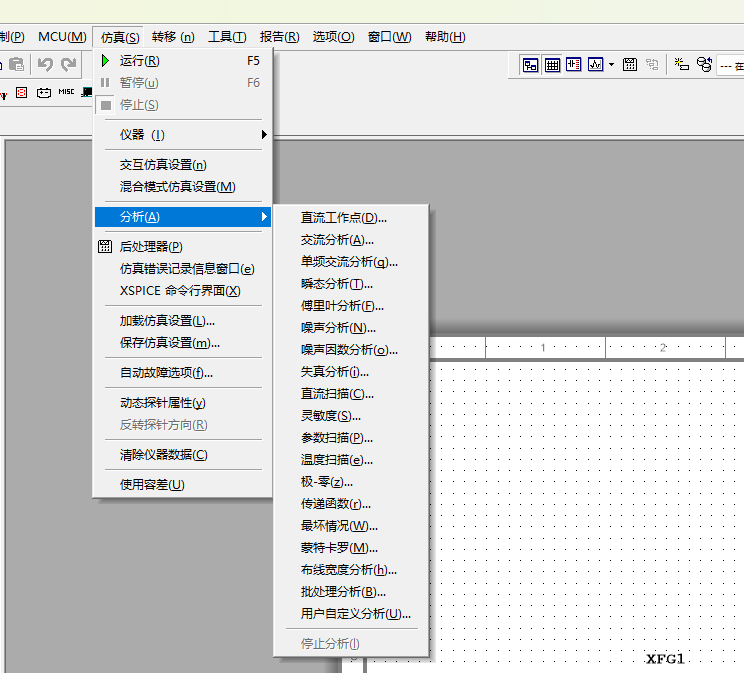
\includegraphics[width=0.5\textwidth]{5.2.3_1}	
\end{figure}

直流工作点分析:
\begin{figure}[H]
	\centering
	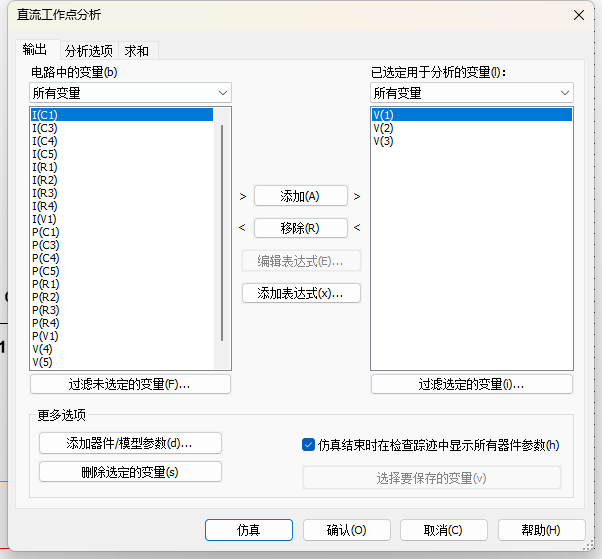
\includegraphics[width=0.5\textwidth]{5.2.3_2}	
\end{figure}

直流工作点分析是在电路电感短路,电容开路的情况下,计算电路的静态工
作点 。直流分析的结果通常可用于电路的进一步分析,如在进行交流小信号分析前,先分析直流工作点,以确定交流小信号放大的条件是否满足。用户可以选择输出想要的得到的电压和电流。

交流分析:
\begin{figure}[H]
	\centering
	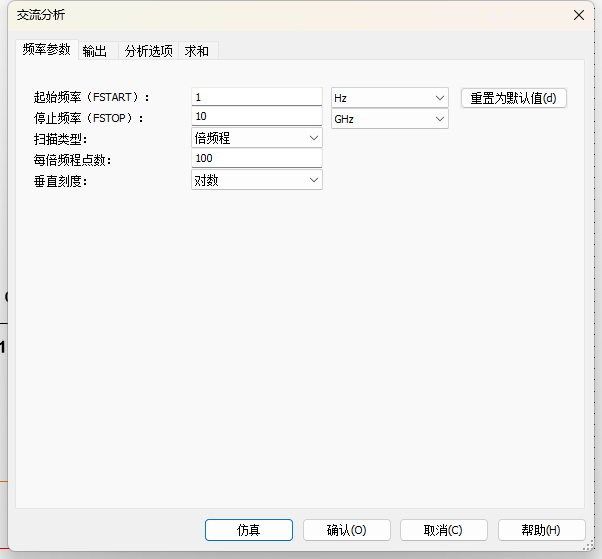
\includegraphics[width=0.5\textwidth]{5.2.3_3}	
\end{figure}

交流分析是分析小信号时的频率响应。分析程序首先对电路进行直流工作点
分析,以便建立电路中非线性 元件的交流小信号模型, 并且将直流信号源接地,交流信号源、电容及其它器件采用交流模型分析。可以设置交流分析的起始频率和终止频率。还能设置设置交流分析的扫描方式,包含Decade(十倍频扫描)、 Octave(八倍频 扫描)和 Linear(线性扫描),通常选择 Decade 选项,以对数方式显示。

瞬态分析:
\begin{figure}[H]
	\centering
	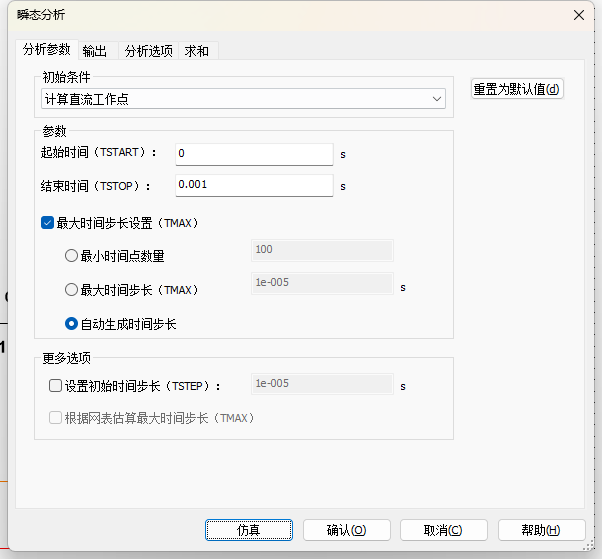
\includegraphics[width=0.5\textwidth]{5.2.3_4}	
\end{figure}

瞬态分析是一种时域分析,可以在激励信号的情况下计算电路的时域响应。
分析时,电路的初始状态可由用户自行指定, 也可以由程序进行直流分析后解出电路初始状态。

\section{实验过程}
\subsection{Multisim 仿真}
\subsubsection{DC Operating Point 模拟直流静态工作点}
电路图如下:
\begin{figure}[H]
	\centering
	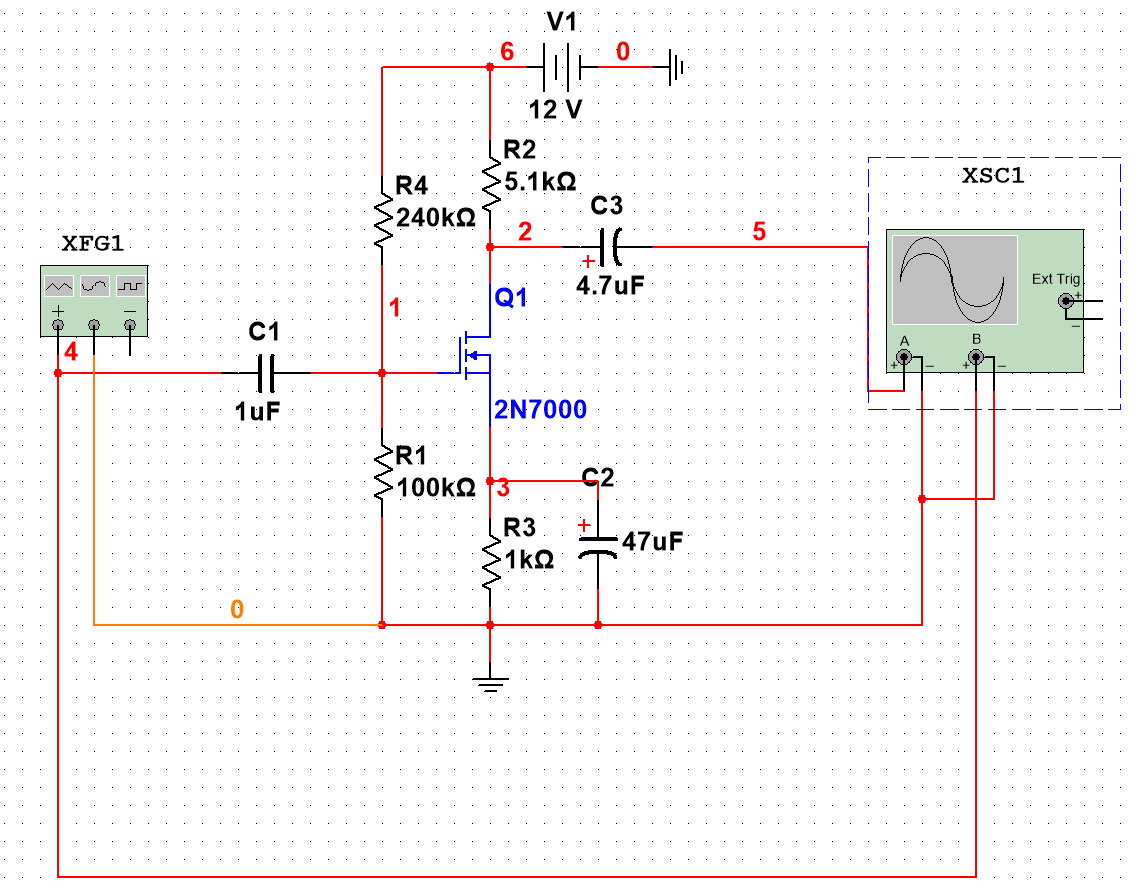
\includegraphics[width=0.7\textwidth]{2.4.PNG}	
\end{figure}
测量静态工作点,选择直流工作点分析,得到此时对应的直流工作点:
\begin{figure}[H]
		\subfigure{
		\centering
		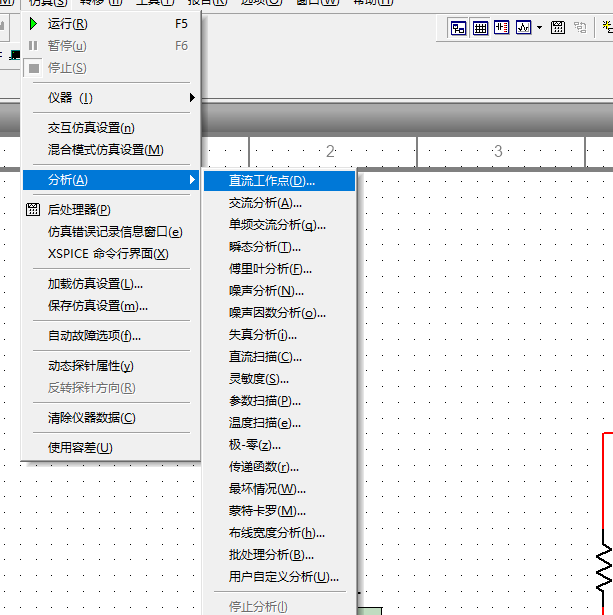
\includegraphics[width=0.49\textwidth]{Q_pt}	
	}
	\subfigure{
		\centering
		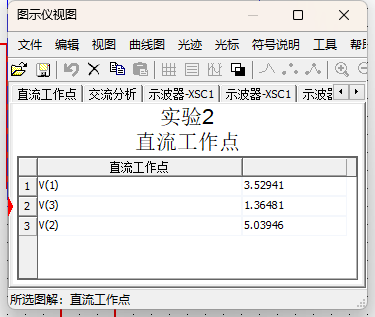
\includegraphics[width=0.49\textwidth]{2.5.PNG}	
	}

\end{figure}
\subsubsection{Single frequency ac analysis 得到输入输出电压曲线}
通过观测示波器XSC1的输出,可以得到输出输入曲线,其中光标标记了输入输出的幅值,可以计算得到放大倍数约为87.56
\begin{figure}[H]
	\centering
	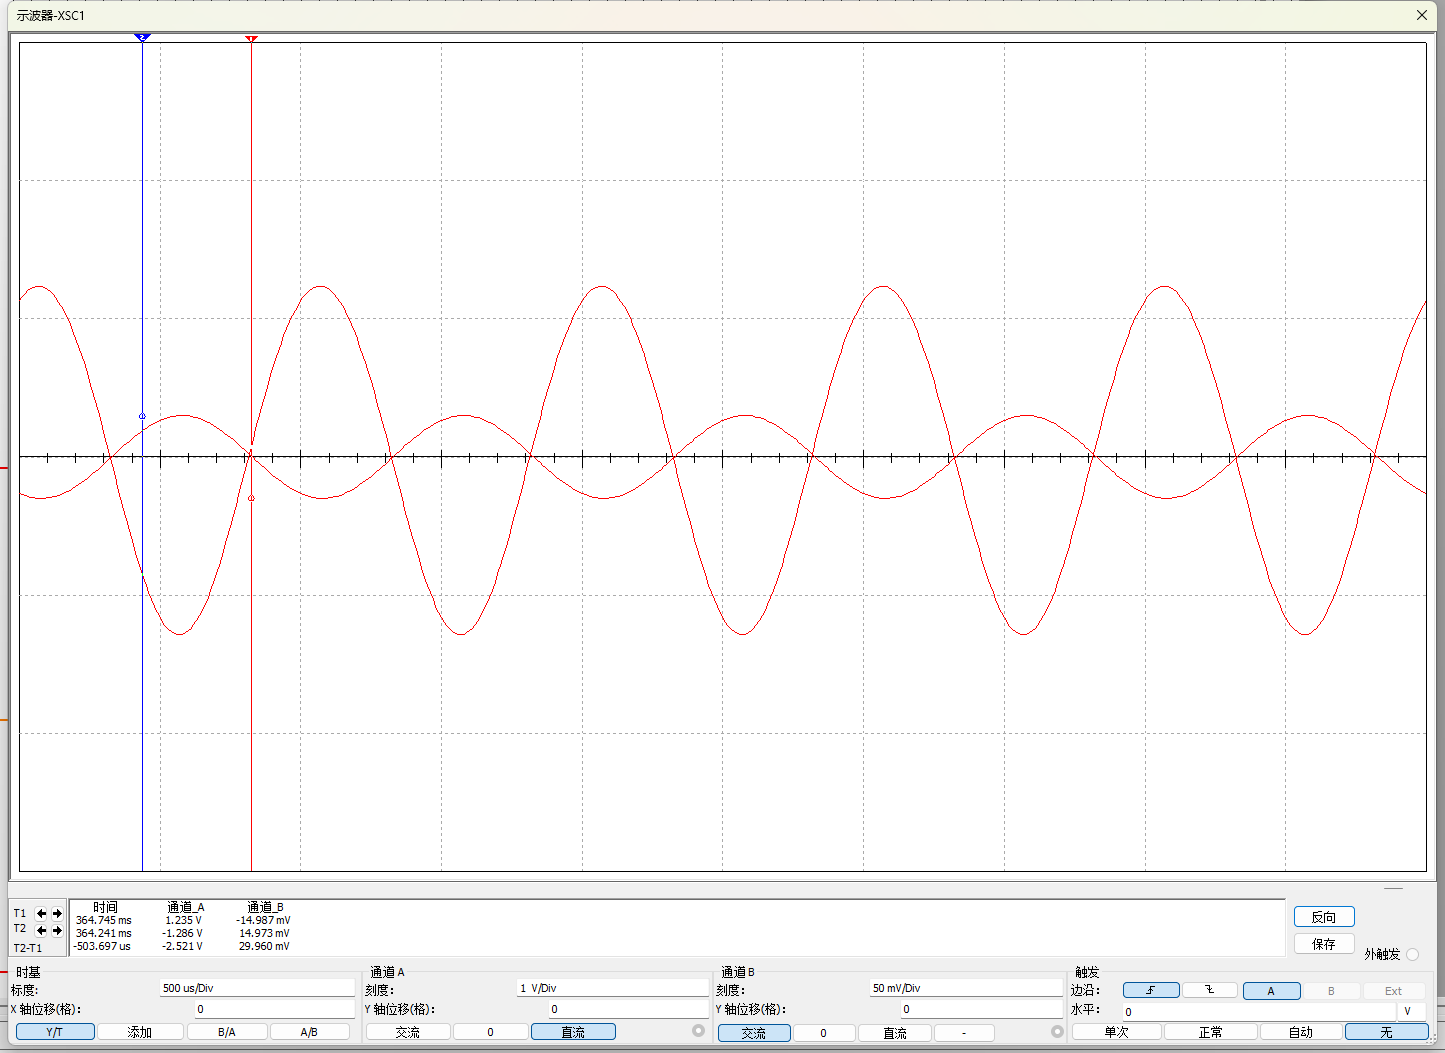
\includegraphics[width=0.9\textwidth]{2.6.PNG}	
\end{figure}
接入$R_L$之后,电路图如下:
\begin{figure}[H]
	\centering
	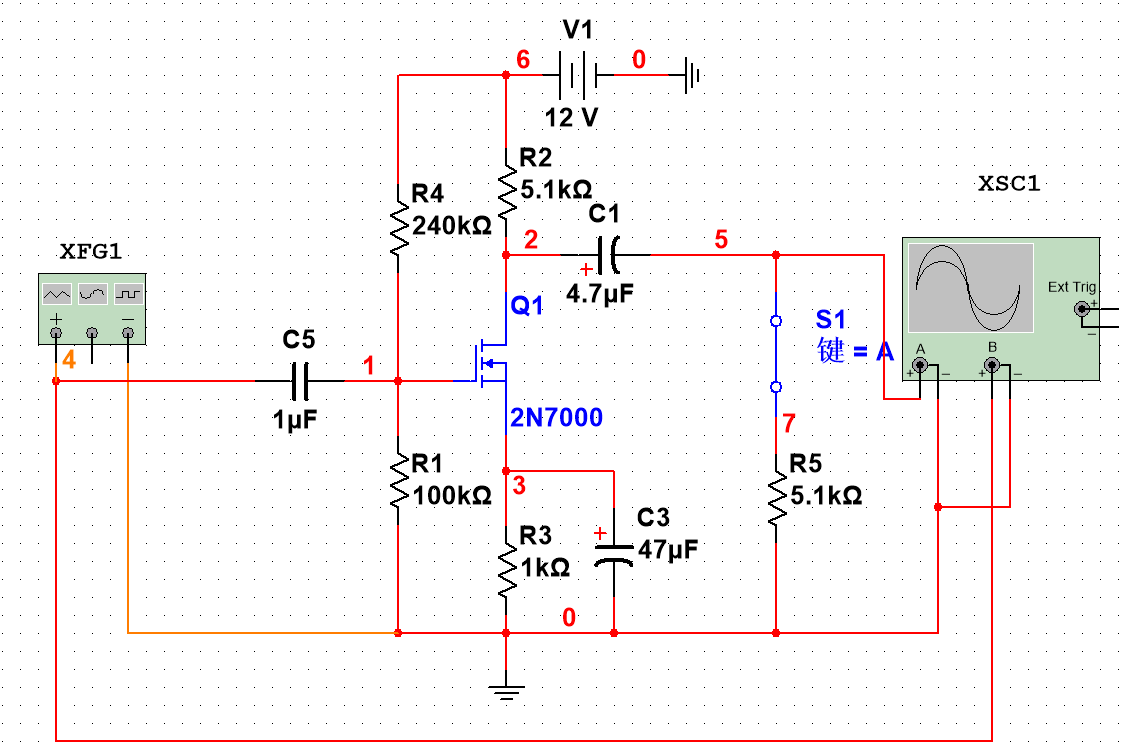
\includegraphics[width=0.9\textwidth]{6.1.2.PNG}	
\end{figure}
再次通过观测示波器XSC1的输出得到输出输入曲线,计算得到放大倍数约为43.99,波形如下:
\begin{figure}[H]
\centering
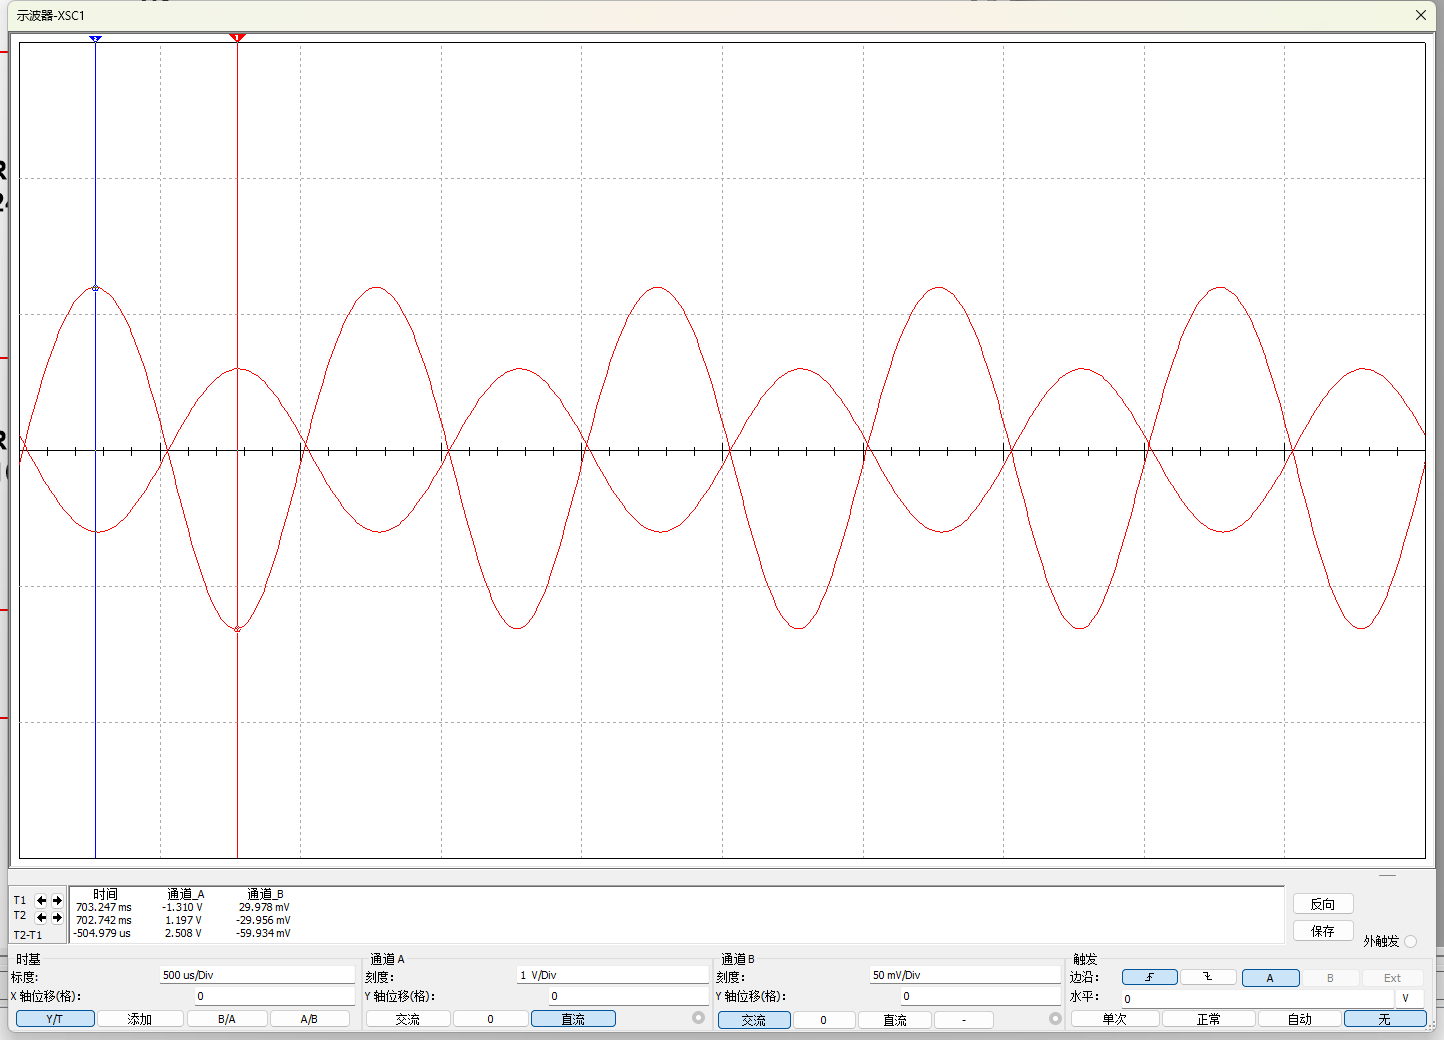
\includegraphics[width=0.8\textwidth]{VoR_L.PNG}	
\end{figure}
\subsubsection{AC Analysis 得到幅频特性曲线}
在分析中选择交流分析,垂直刻度设置为线性,输出设置为$dB(v_o/v_i)$:
\begin{figure}[H]
	\subfigure{
		\centering
		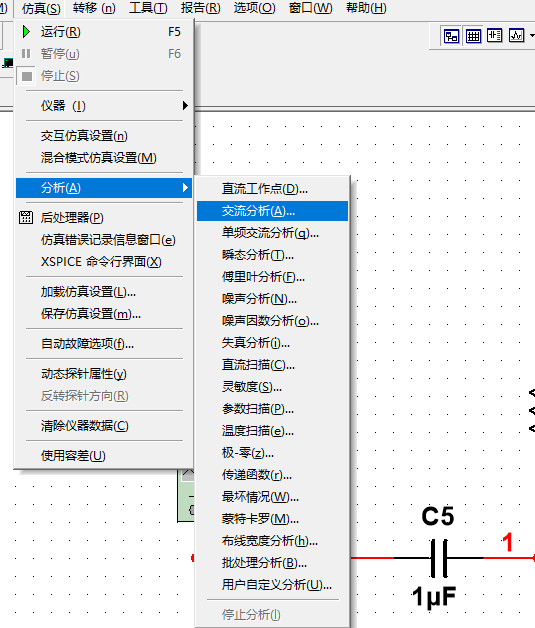
\includegraphics[width=0.3\textwidth]{6.1.3_1.PNG}	
	}
	\subfigure{
		\centering
		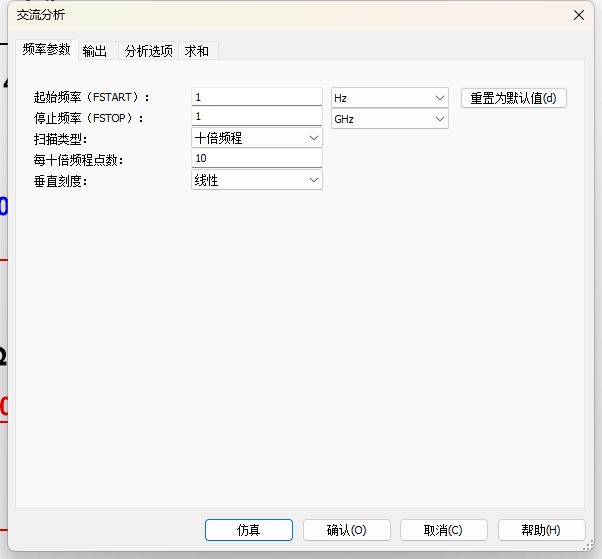
\includegraphics[width=0.3\textwidth]{6.1.3_2.PNG}	
	}	
	\subfigure{
		\centering
		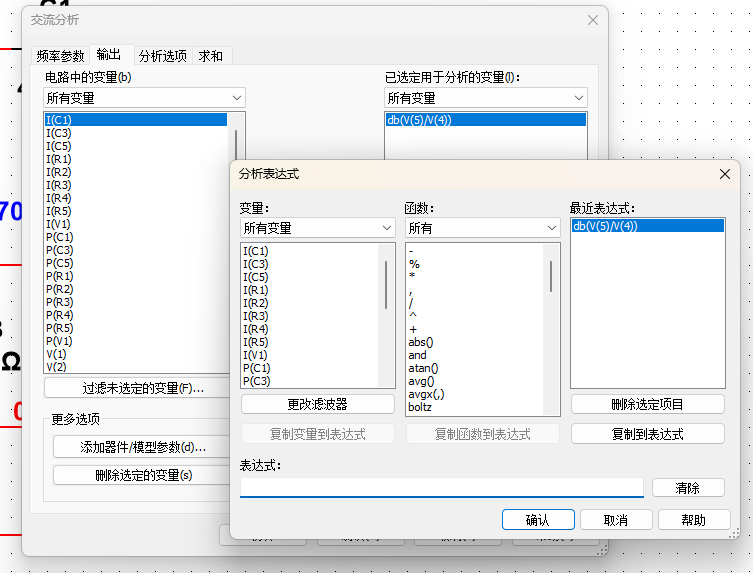
\includegraphics[width=0.3\textwidth]{6.1.3_4.PNG}	
	}
\end{figure}
已知通频带增益为38.5209左右,下图光标标记了-3dB处的上下限频率:
\begin{figure}[H]
	\centering
	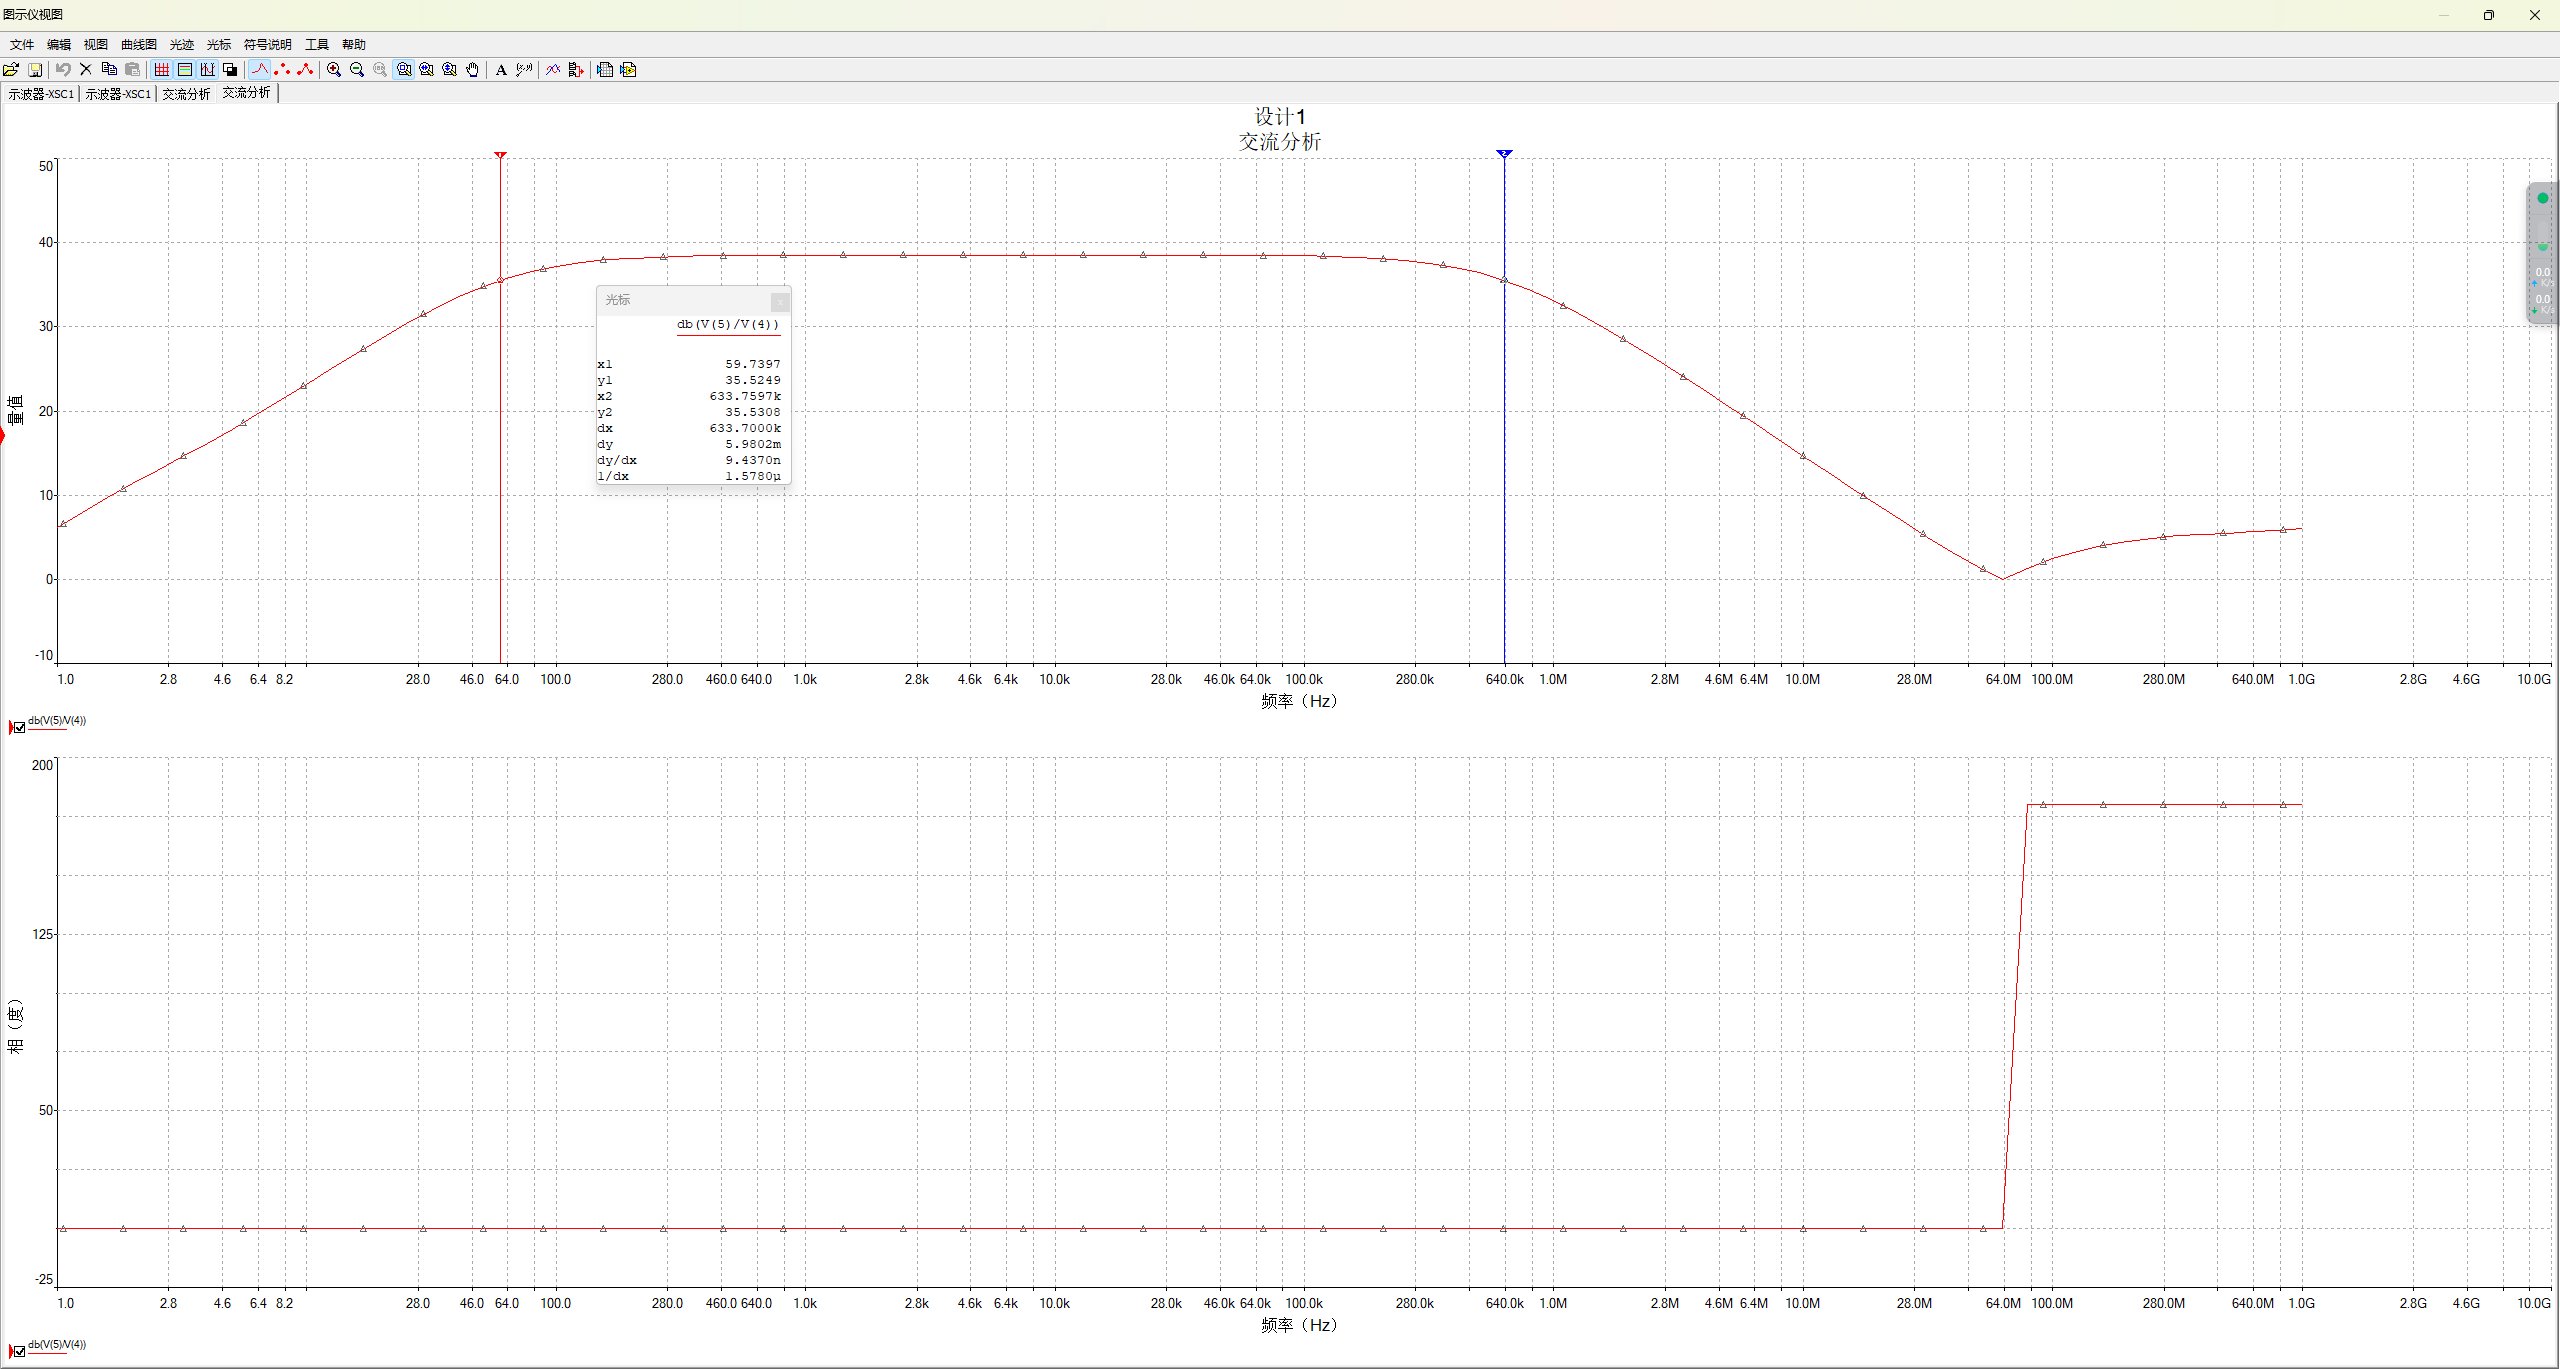
\includegraphics[width=1\textwidth]{6.1.3_3.PNG}	
\end{figure}
可以得到上下限频率:$f_L=59.7397$Hz,$f_H=633.7597$kHz
\subsubsection{AC 模式测量输入阻抗}
在分析中选择交流分析,垂直刻度设置为线性,输出设置为$v_o/i_{C5}$,可以得到输入电阻-频率曲线:
\begin{figure}[H]
	\centering
	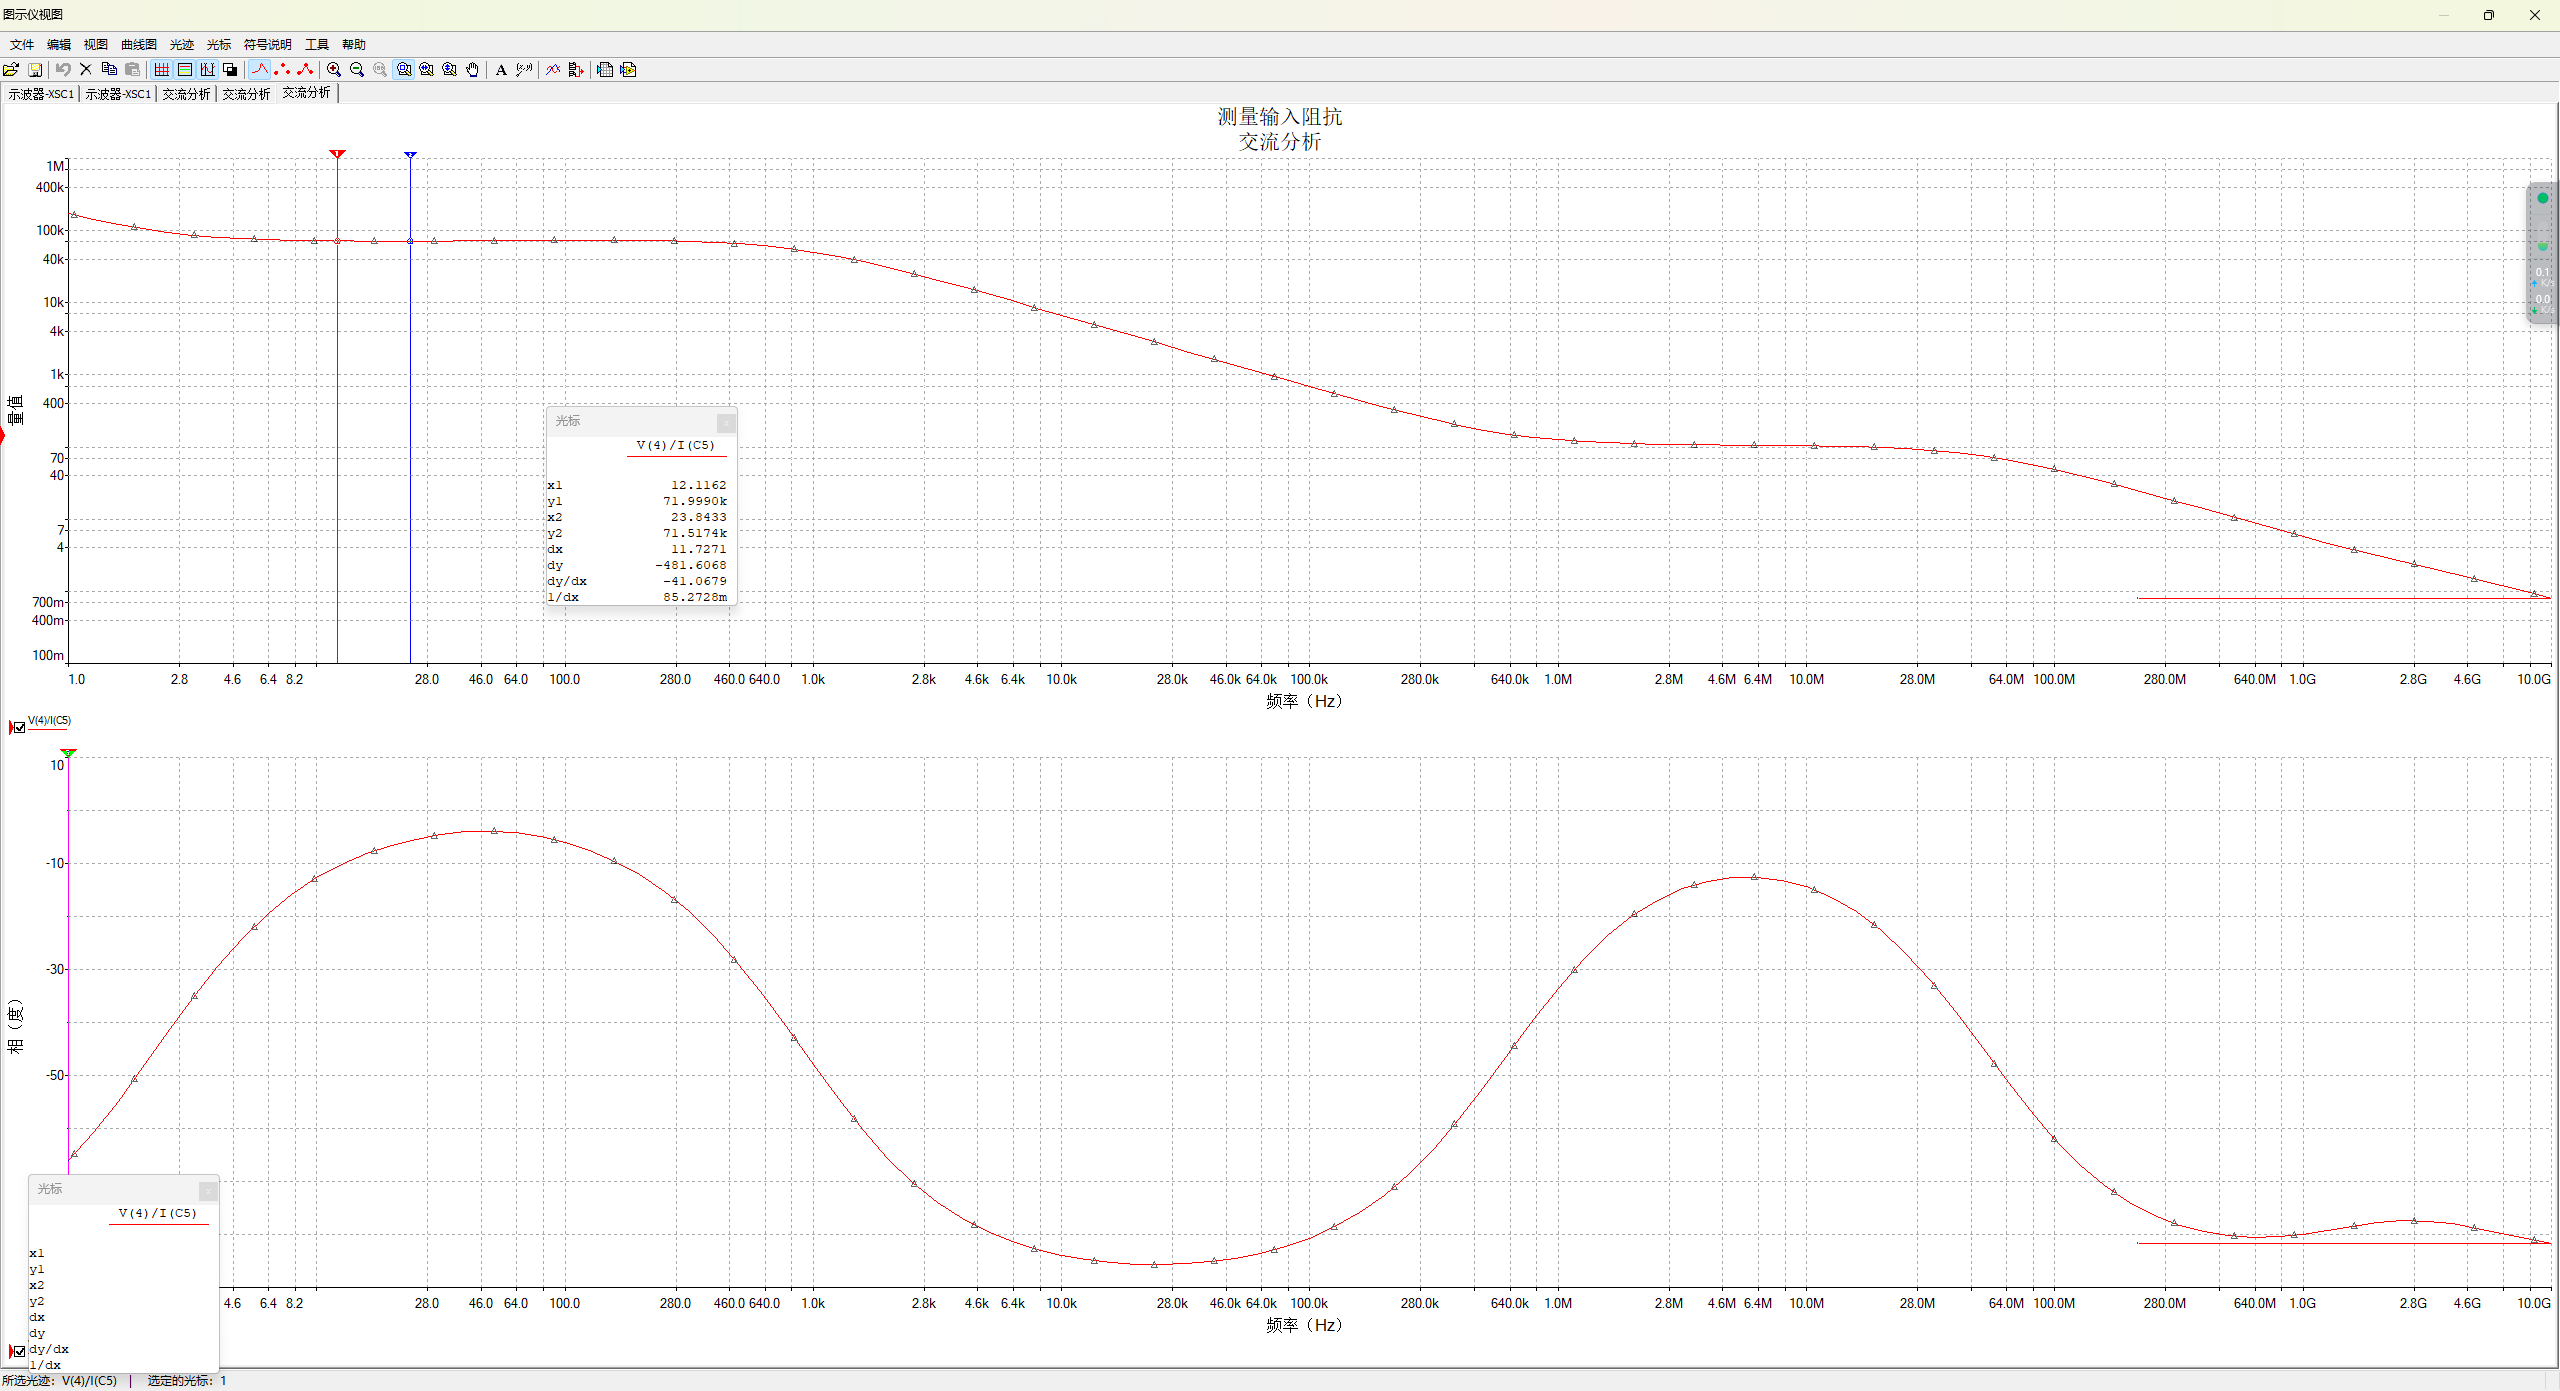
\includegraphics[width=1\textwidth]{6.1.4_1.PNG}	
\end{figure}
根据光标可以观察到$R_i=71.5174\mathrm{k\Omega}$
\subsubsection{AC 模式测量输出阻抗}
输出电阻的测量略有不同,需要调整为在输入短路的条件下在输出端加压限流的方式计算$v_o/v_i$,修改的电路图如下:
\begin{figure}[H]
	\centering
	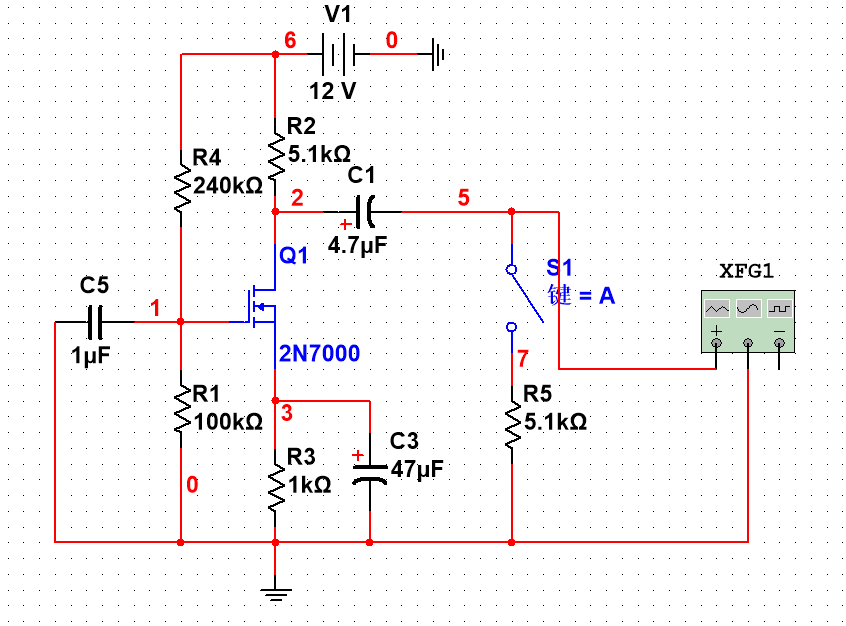
\includegraphics[width=0.8\textwidth]{6.1.5_1.PNG}	
\end{figure}
输出电阻-频率曲线如下:
\begin{figure}[H]
	\centering
	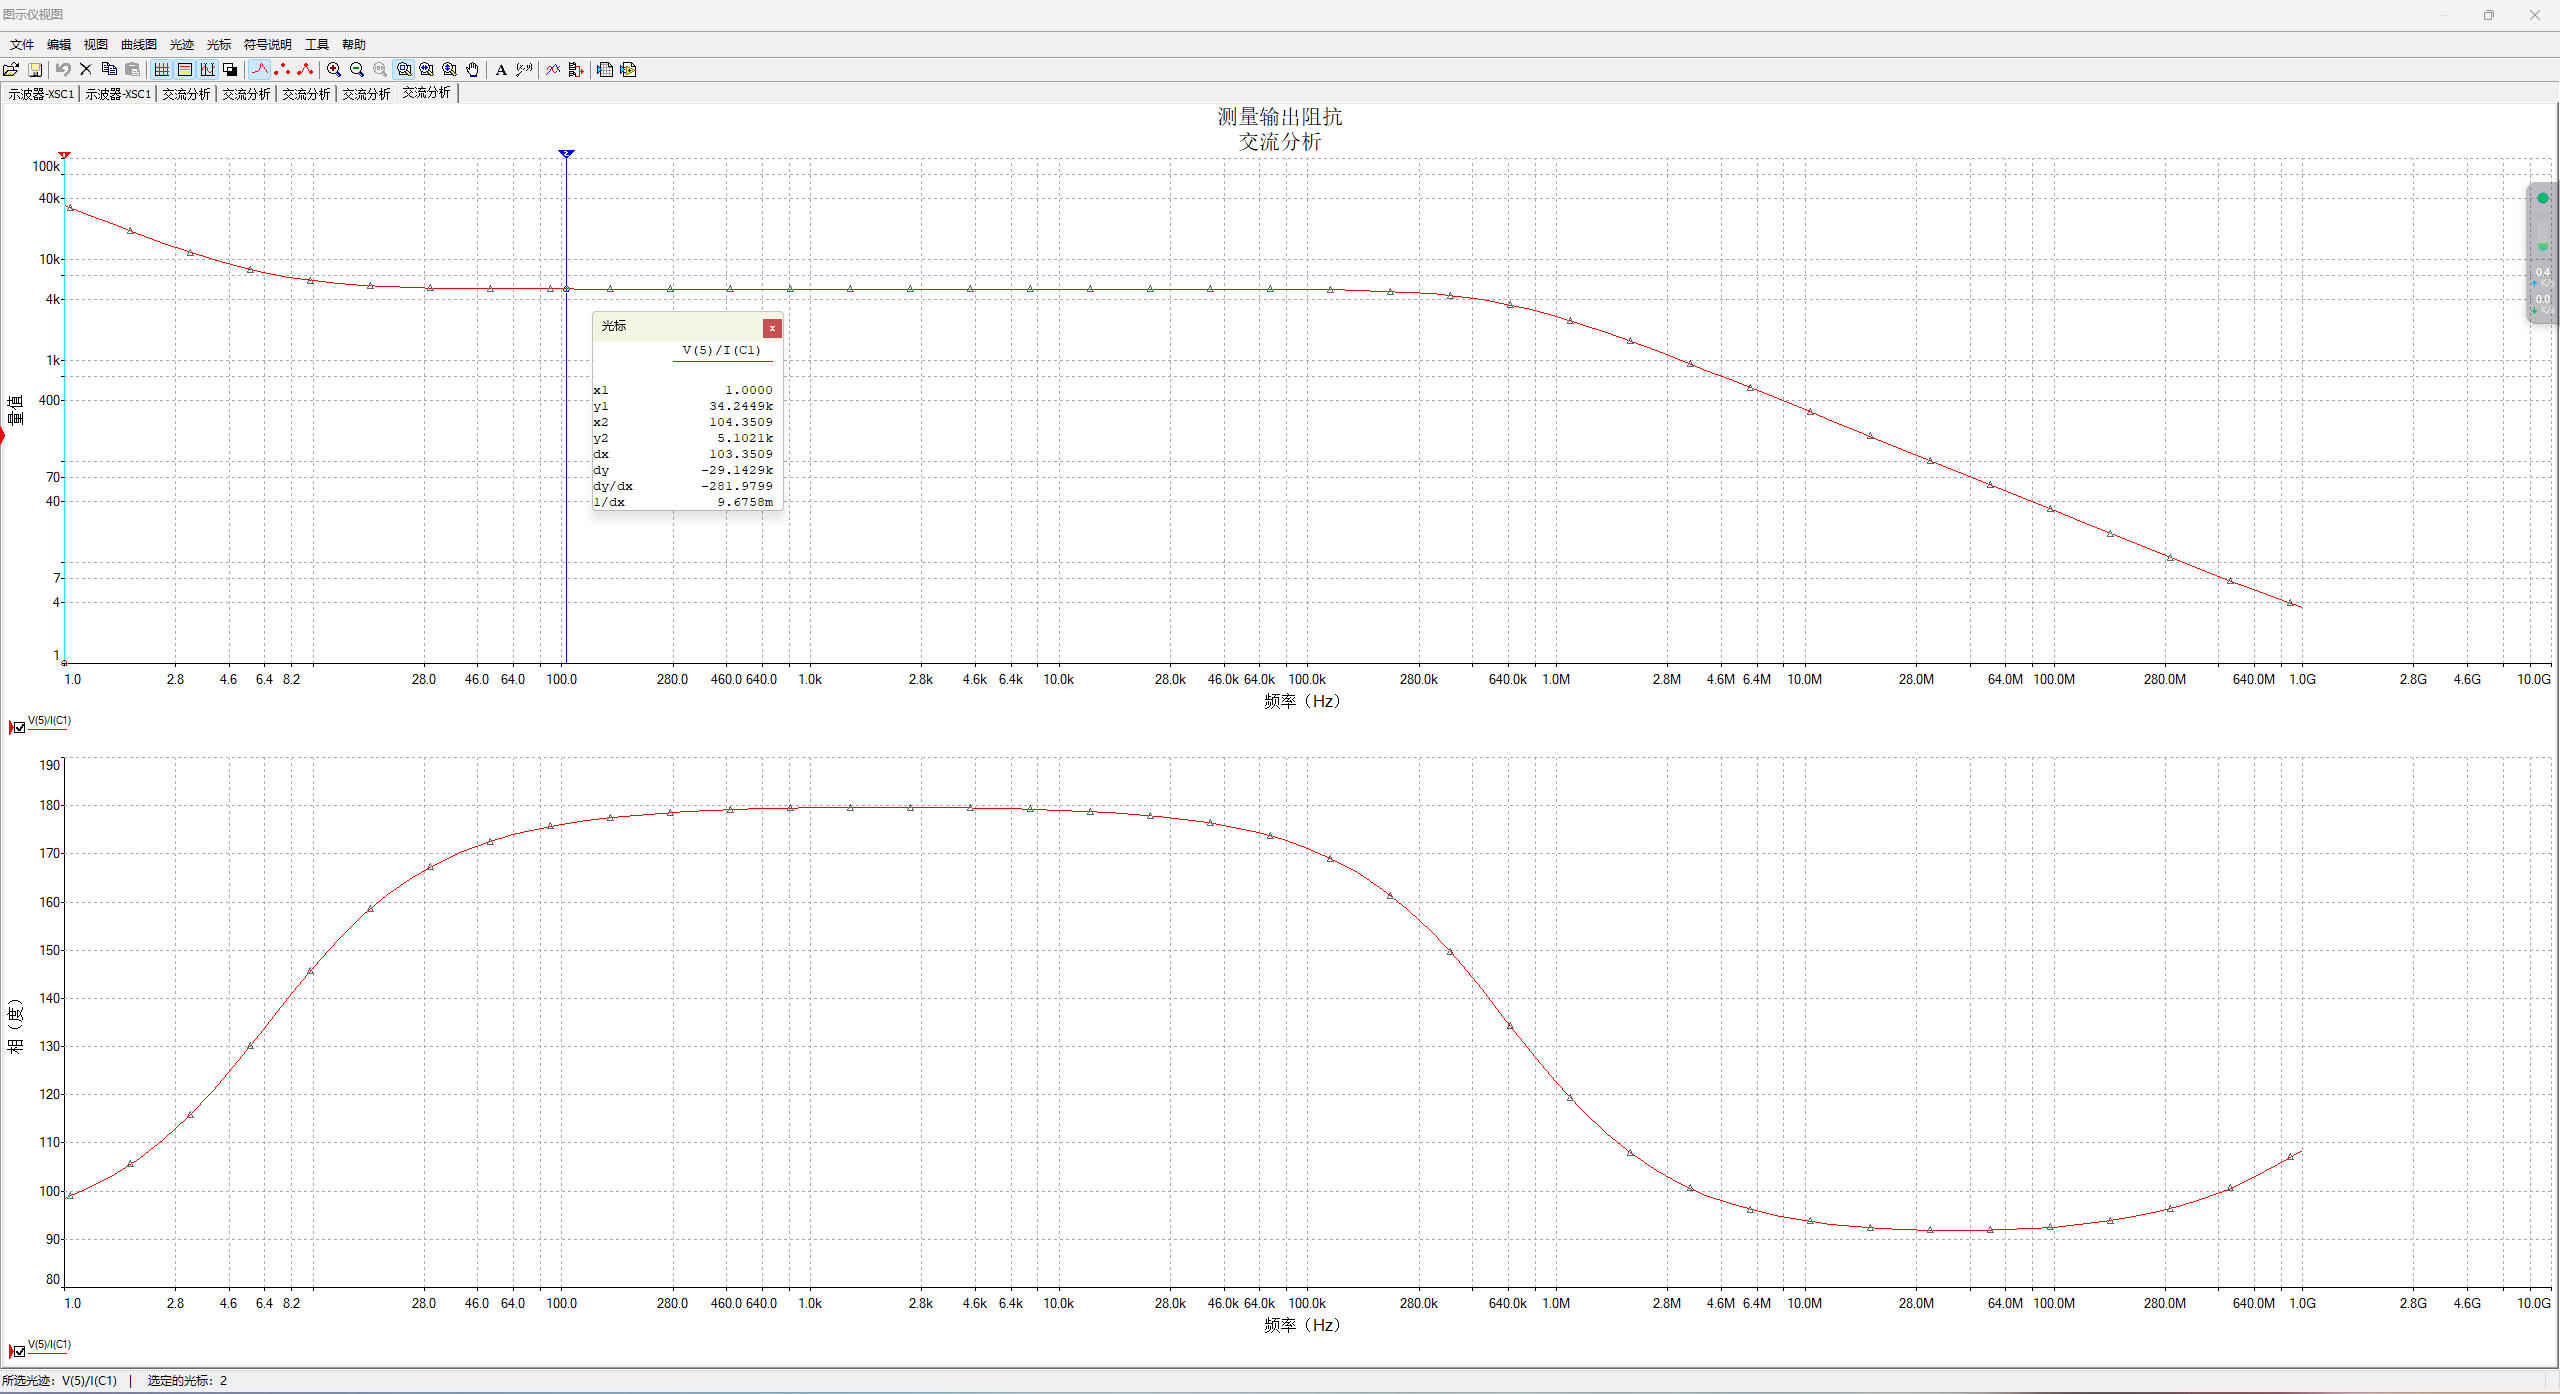
\includegraphics[width=1\textwidth]{6.1.5_2.PNG}	
\end{figure}
根据光标可以观察到$R_o=5.1021\mathrm{k\Omega}$
\subsection{单极 MOSFET 共源放大电路插板实验}
\subsubsection{测试静态工作点}
实验中数据记录表格如下:
\begin{table}[H]
	\centering
	\resizebox{\linewidth}{!}{\begin{tabular}{|c|c|c|c|c|c|c|c|}
			\hline
			\multirow{2}{*}{} & \multicolumn{3}{c|}{实测值} & \multicolumn{3}{c|}{计算值} & \multirow{2}{*}{\shortstack{MOSFET处于\\哪个工作区}}\\
			\cline{2-7}
			& $V_{G}$/V & $V_{S}$/V & $V_{D}$/V & {$I_{DQ}=V_S/R_S$/mA}& $V_{GSQ}=(V_G-V_S)$/V & $V_{DSQ}=(V_D-V_S)$/V & \\
			\hline
			\makecell[l]{$R_{g1}=240k$\\$R_{g2}=100k$} & 3.4517 & 1.8518 & 2.5901 & 0.3692 & 1.5999 & 0.7383& Nonsaturation \\	
			\hline
			\makecell[l]{$R_{g1}=100k$\\$R_{g2}=100k$} & 5.9946 & 1.9732 & 1.9803 & 0.3934 & 4.0214 & 0.0071 & Nonsaturation\\	
			\hline
			\makecell[l]{$R_{g1}=240k$\\$R_{g2}=33k$} & 1.4417 & 0.16356 & 11.4622 & 0.2874 & 1.27814 & 11.27814 & Cut-off\\
			\hline
			实测电阻值 &\multicolumn{7}{c|}{$R_{g1}=241.87\mathrm{k\Omega},97.839\mathrm{k\Omega}$,$\qquad R_{g2}=98.232\mathrm{k\Omega},33.132\mathrm{k\Omega}$,$\qquad R_{d}=5.0156k\Omega$,$\qquad R_{s}=983.44\Omega\qquad$}\\
			\hline				
		\end{tabular}
	}
	\caption{静态工作点}
\end{table}
\subsubsection{测试放大电路的输入、输出波形和通带电压增益}
输入、输出波形如下:
\begin{figure}[H]
	\subfigure{
		\centering
		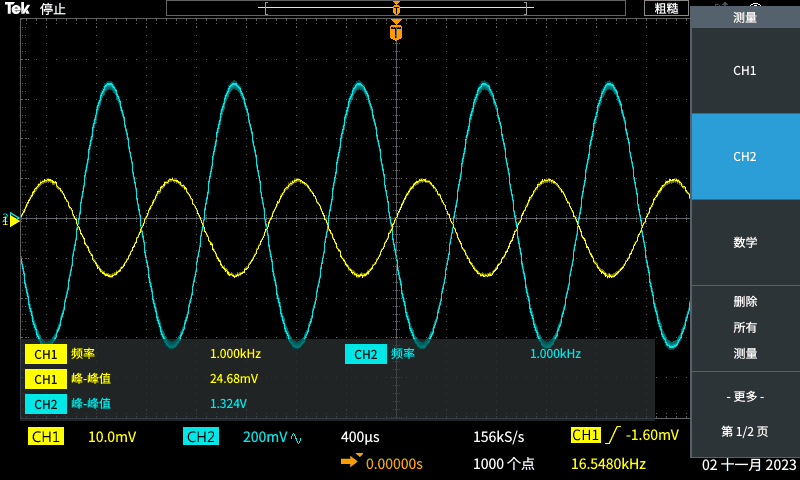
\includegraphics[width=0.49\textwidth]{TEK00013.PNG}
	}
	\subfigure{
		\centering
		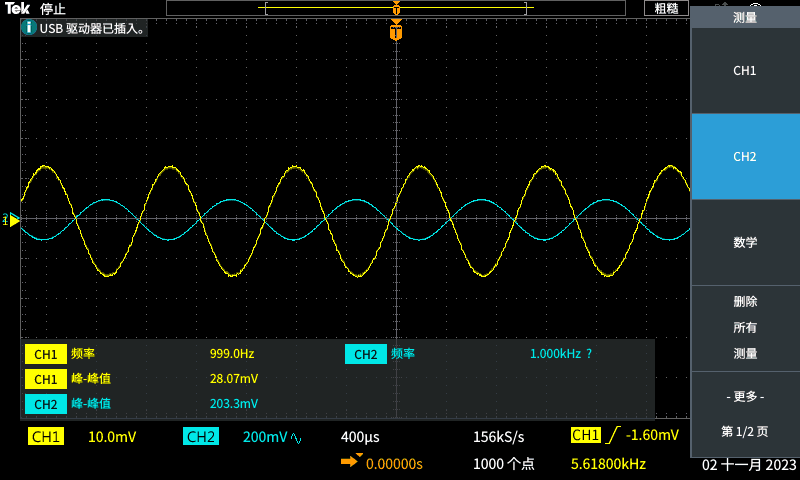
\includegraphics[width=0.49\textwidth]{TEK00014.PNG}
	}
\end{figure}
实验数据记录表格如下:
\begin{table}[H]
	\centering
	\begin{tabular}{|c|c|c|c|c|c|}
			\hline
			\shortstack{负载\\情况} & \shortstack{$v_i$峰-峰\\值$V_{ipp}$/mV} & \shortstack{$v_o$峰-峰值\\$V_{opp}$/mV} & \shortstack{$|A_v|=$\\$V_{opp}/V_{ipp}$}	& \shortstack{$|A_v|$的\\理论值} & \shortstack{相对\\误差}\\
			\hline
			负载开路 & 30(24.68) & 1304& 52.83& 87.56 & 40.27\%\\
			\hline
			$R_L=5.1\mathrm{k\Omega}$ & 30(28.07) & 203.3 & 7.24 & 10.95 &33.88\%\\
			\hline		
		\end{tabular}
	\caption{:电压增益($f\mathrm{=}\mathrm{1kHz}$)}
\end{table}
\subsubsection{测试放大电路的输入电阻}
测量得到此时的$R=50.914\mathrm{k\Omega}$,接入电路后,输出波形如下:
\begin{figure}[H]
	\centering
	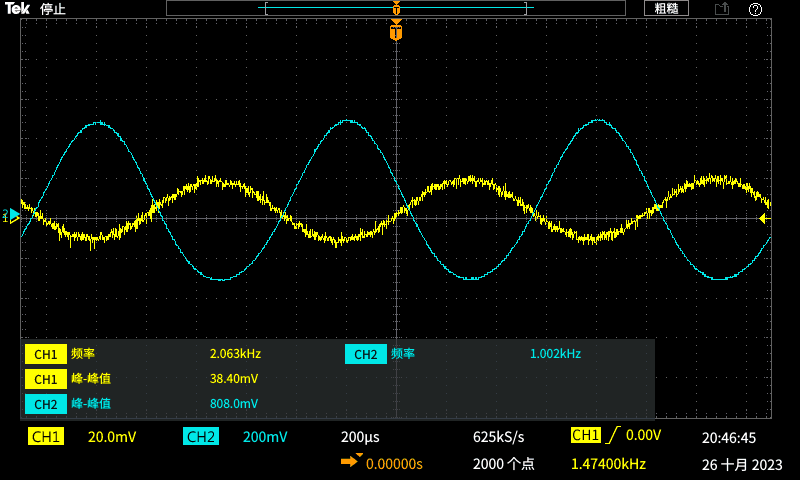
\includegraphics[width=0.7\textwidth]{TEK00009.PNG}
\end{figure}

根据公式(4.3.1)可以计算输入电阻为:$R_i=82.94\mathrm{k\Omega}$
\subsubsection{测试放大电路的输出电阻}
测量得到此时的$R_L=4.9449\mathrm{k\Omega}$,根据表4以及公式(4.3.2)可以计算输出电阻为:$R_o=4.2740\mathrm{k\Omega}$
\subsubsection{测试放大电路的通频带}
下表记录了通频带的测量数据:
\begin{table}[H]
	\centering
	\resizebox{\linewidth}{!}{\begin{tabular}{|c|c|c|c|c|c|c|c|c|c|c|c|c|c|}
		\hline
		$f$/Hz&5&10&15&20&\color{red}30&40&50&70&100&200&500&2k&30k\\	
		\hline
		$V_{opp}$/mV&420.0&260.0&600.0&700.0&\color{red}920.0&1040&1120&1180&1240&1280&1288&1288&1288\\
		\hline
		100k&200k&250k&260k&270k&275k&\color{red}{280k}&285k&290k&300k&310k&330k&350k&370k\\
		\hline
		1240&1080&960.0&940.0&920.0&920.0&\color{red}912.0&900.0&880.0&860.0&840.0&820.0&780.0&760.0\\
		\hline
		400k&450k&500k&600k&800k&1M&&&&&&&&\\
		\hline
		700.0&680.0&640.0&560.0&440.0&360.0&&&&&&&&\\
		\hline
	\end{tabular}}
	\caption{通频带($V_{\mathrm{ipp}}=30$mV)}
\end{table}
下图绘制了通频带曲线:
\begin{figure}[H]
	\centering
	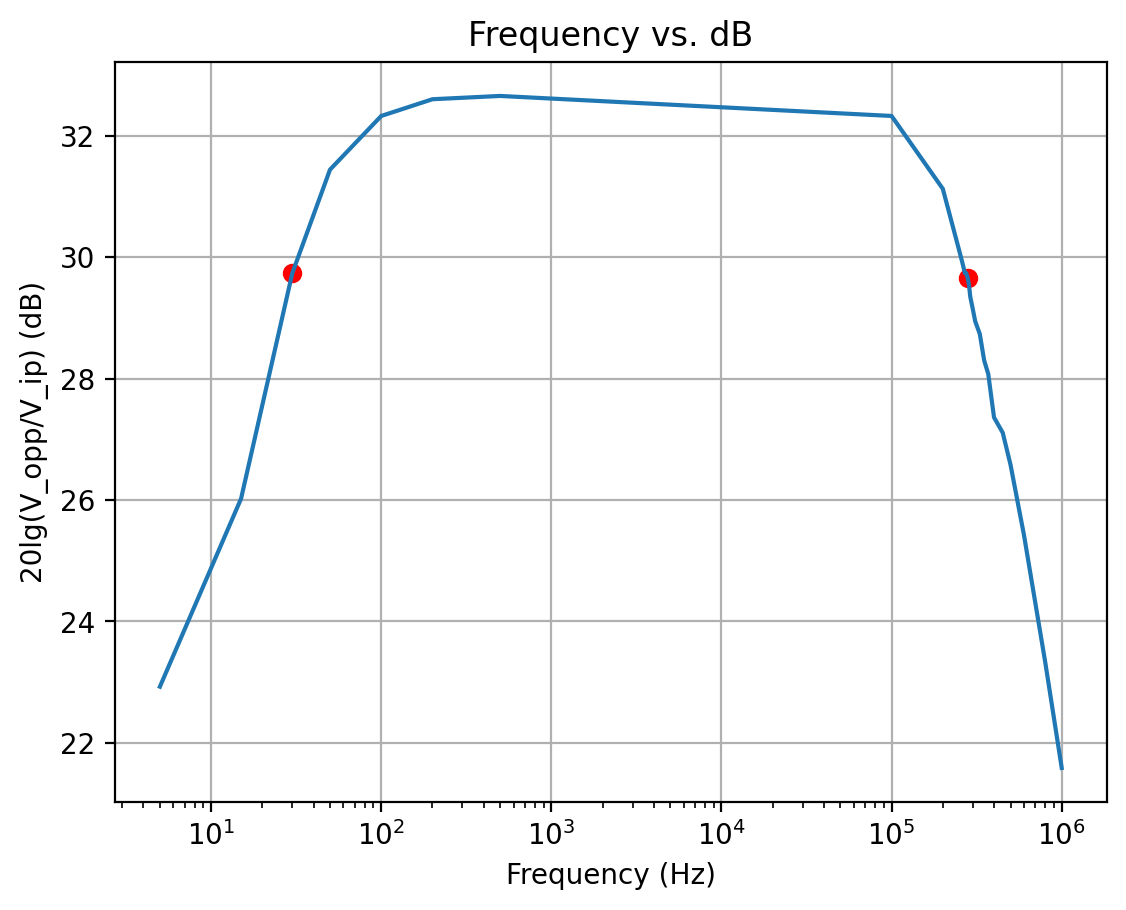
\includegraphics[width=0.7\textwidth]{6.2.5}
\end{figure}
可以得到上下限频率:$f_L=30$Hz,$f_H=280$kHz
\subsection{Multisim 仿真拓展实验}
\subsubsection{MOSFET 输出特性曲线仿真}
电路图如下:
\begin{figure}[H]
	\centering
	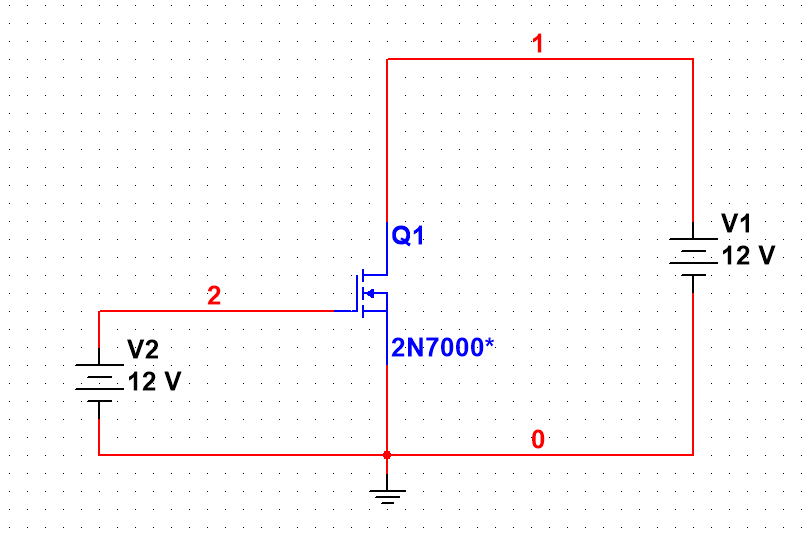
\includegraphics[width=0.4\textwidth]{6.3.1}
\end{figure}
输出特性曲线仿真结果如下:
\begin{figure}[H]
	\centering
	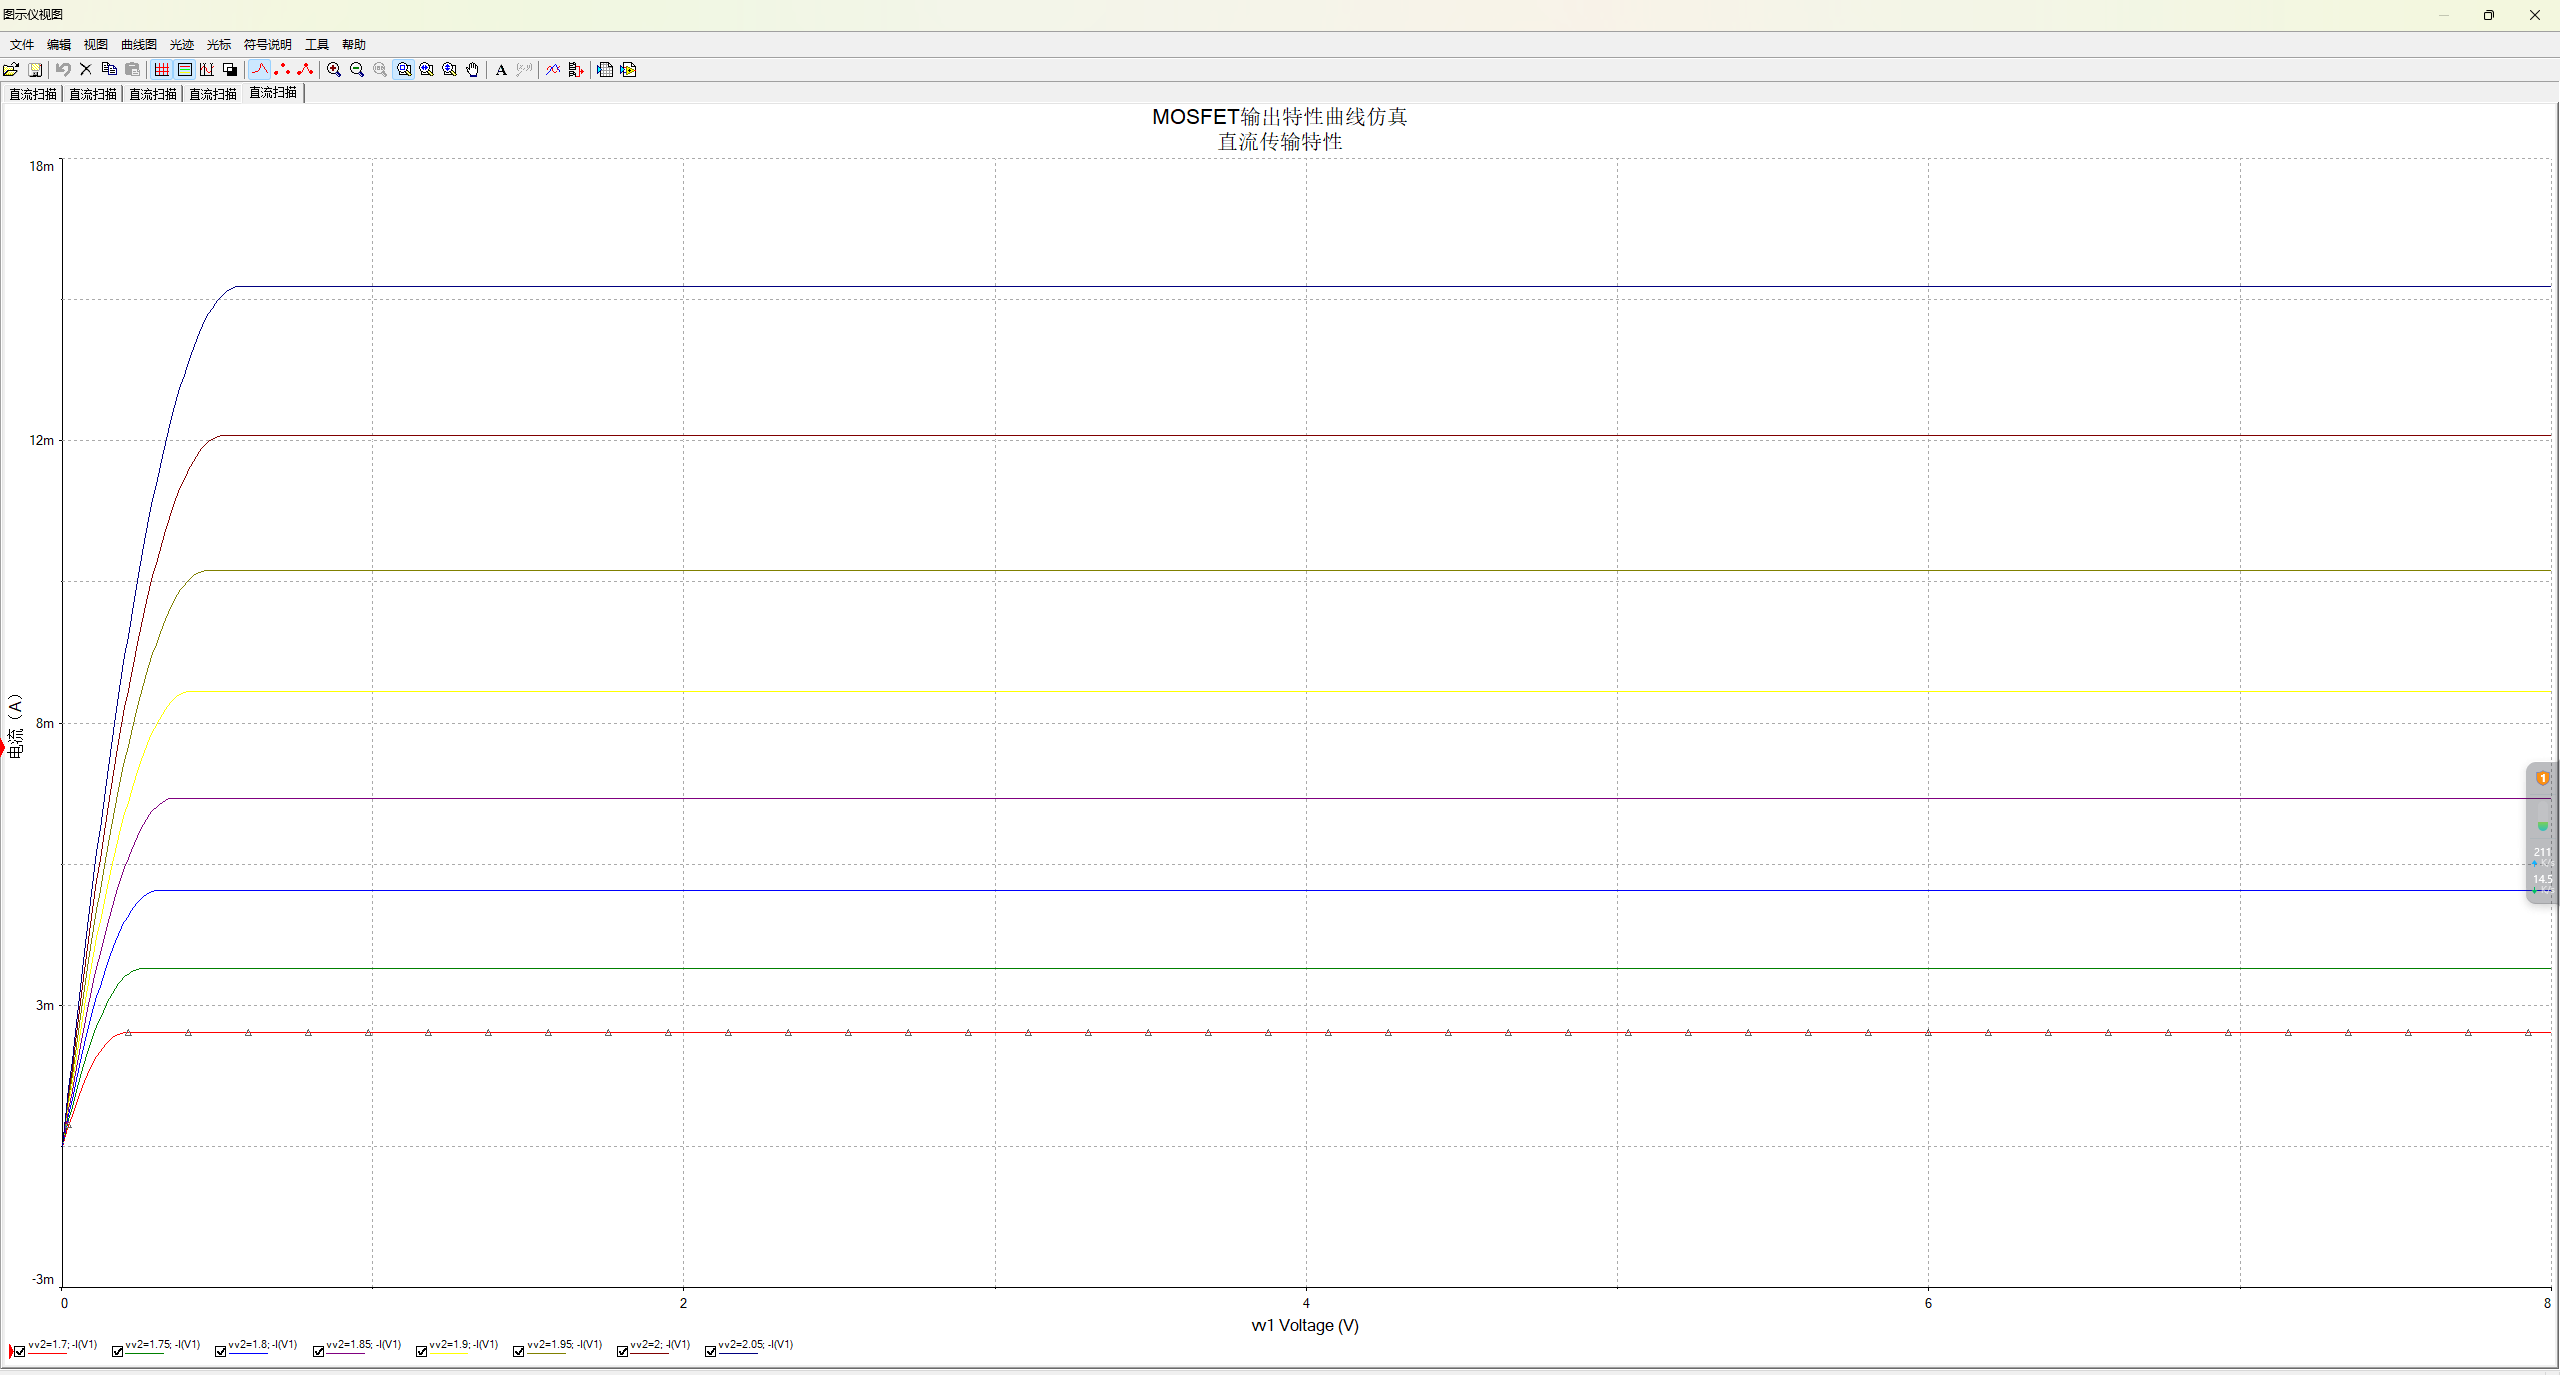
\includegraphics[width=1\textwidth]{6.3.1_1}
\end{figure}
\subsubsection{MOSFET 转移特性曲线仿真}
电路图如下:
\begin{figure}[H]
	\centering
	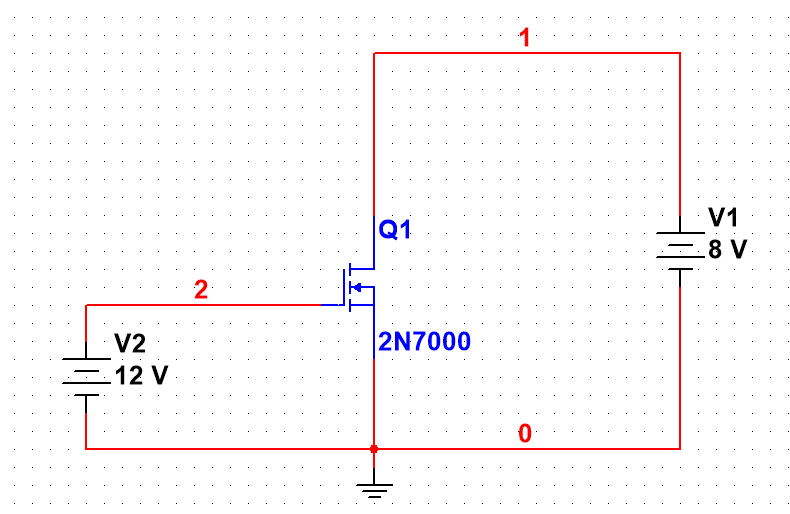
\includegraphics[width=0.4\textwidth]{6.3.2}
\end{figure}
转移特性曲线仿真结果如下:
\begin{figure}[H]
	\centering
	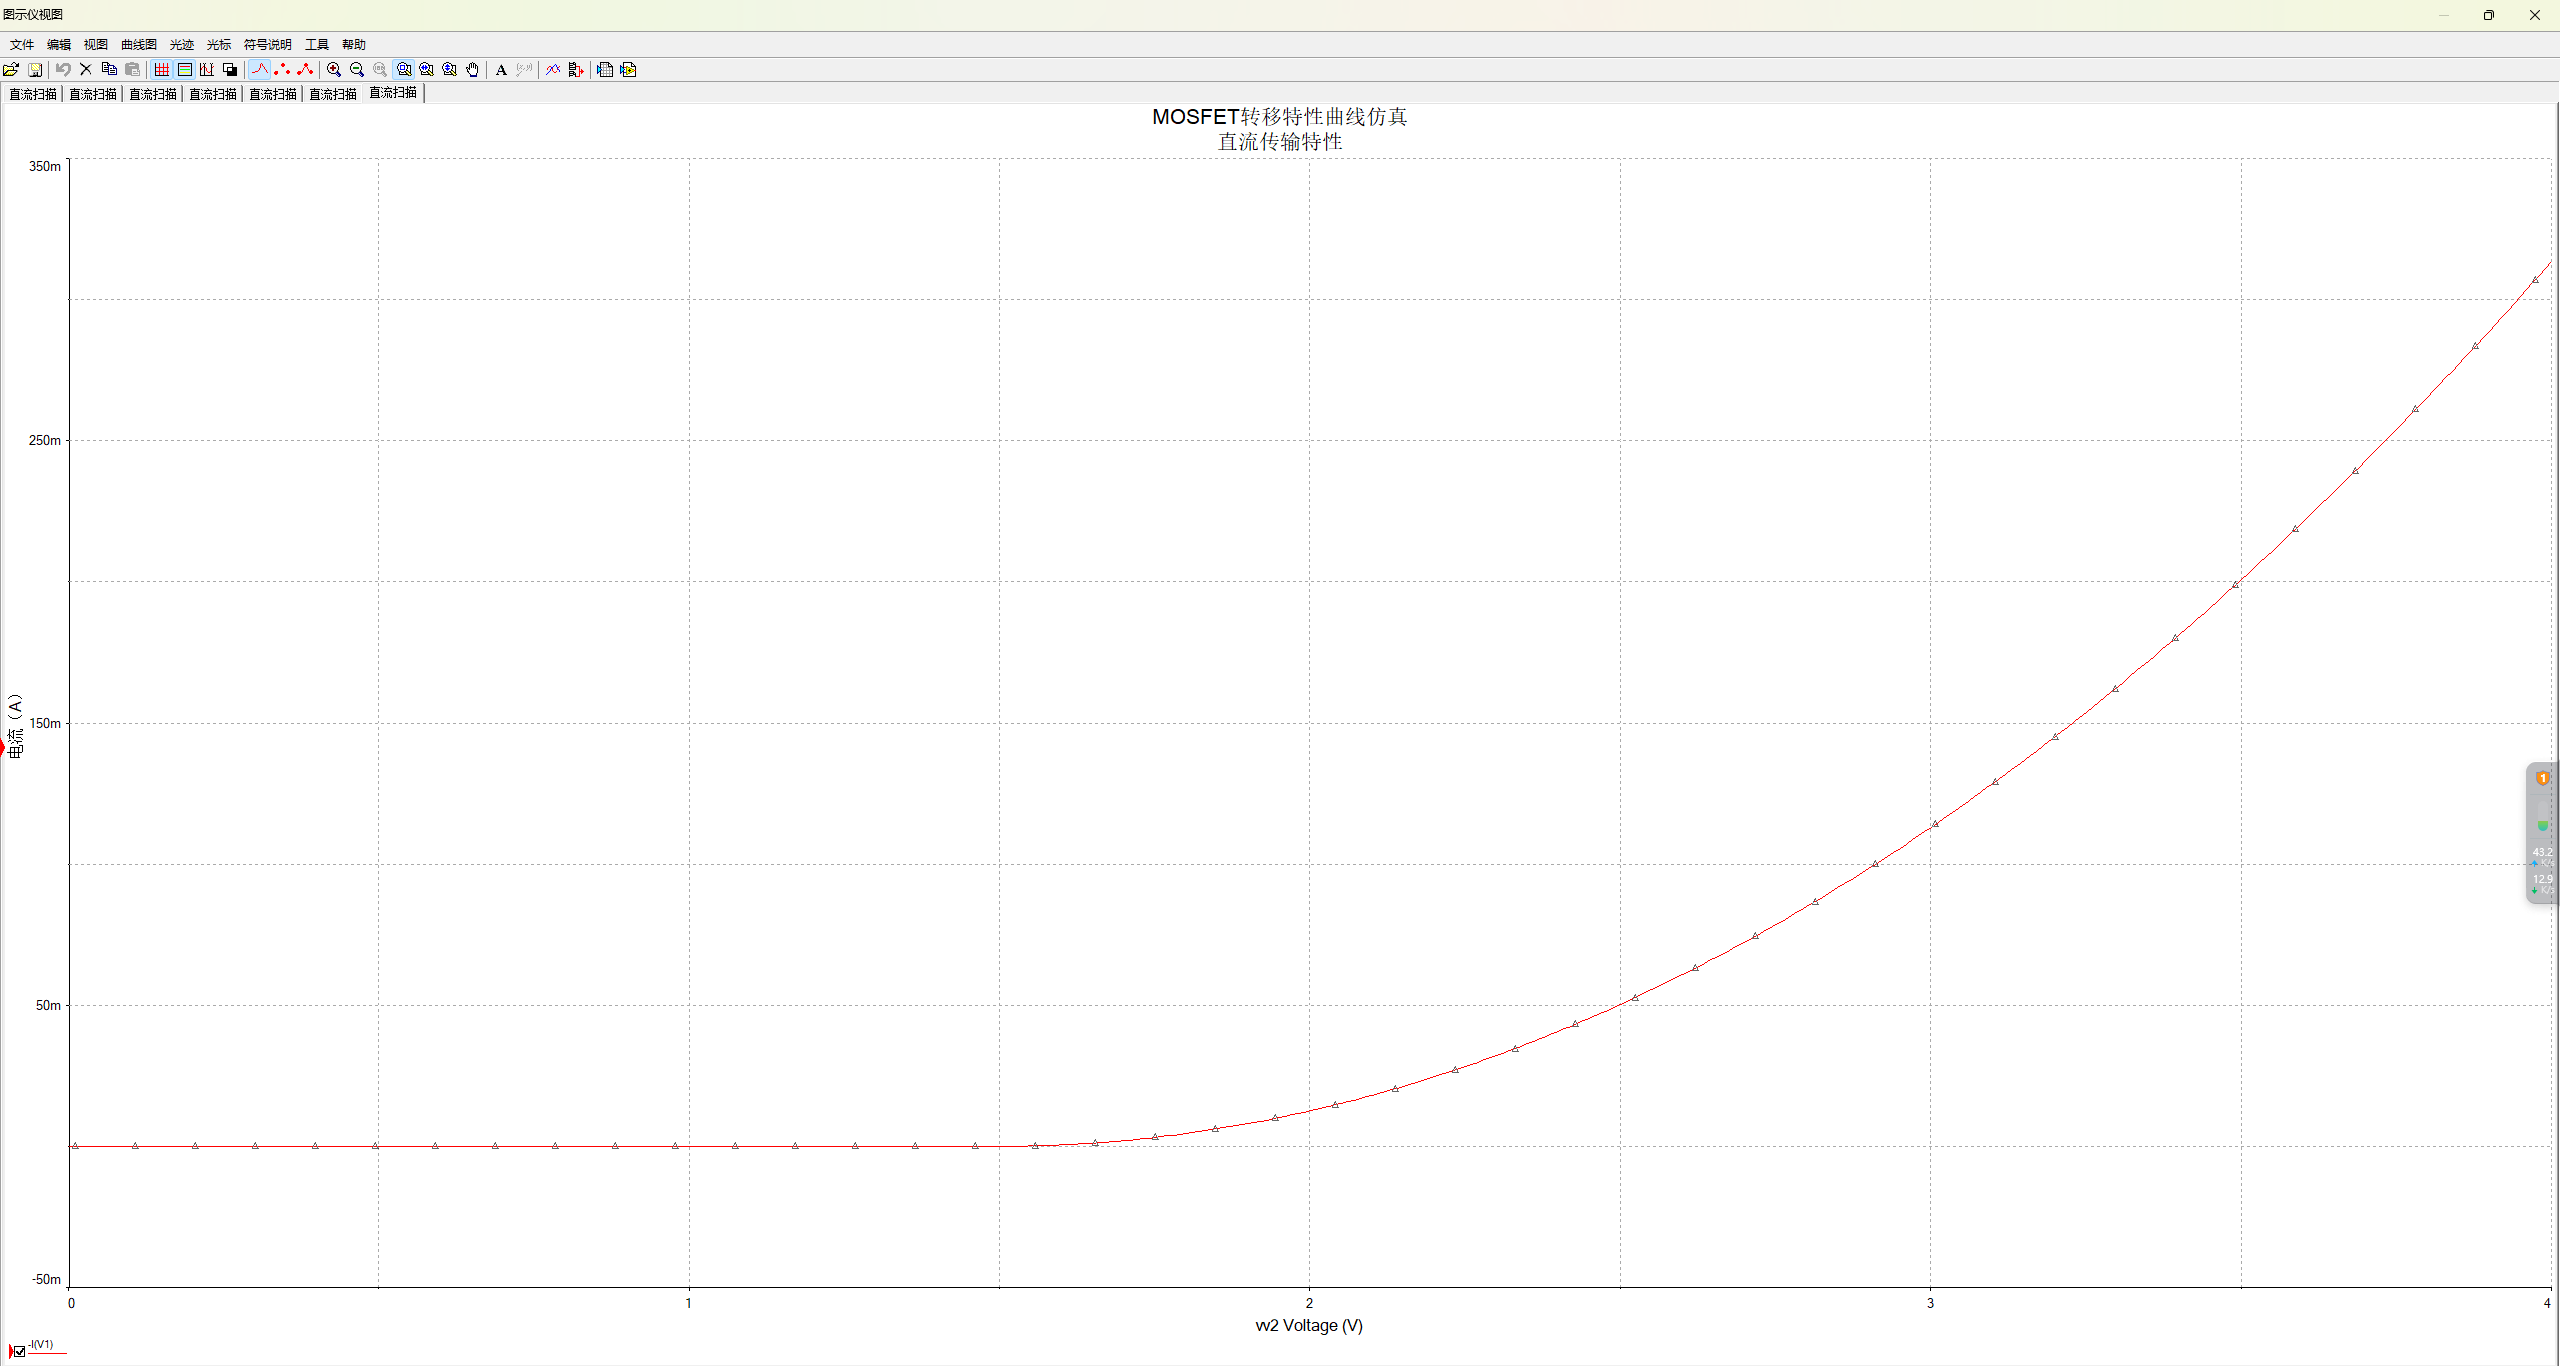
\includegraphics[width=0.9\textwidth]{6.3.2_1}
\end{figure}
\section{实验小结}
本次实验还是遇到了一些小问题。

最重要的一点就是忽略了电解电容的正负极,电解电容接反了导致输出波形有一定失真,这导致我怎么调都没法调出正常波形。上课的时候了解过这个知识点,但是在实际连接线路的时候又给忽略了,接正确后波形就恢复正常了。

其次是仿真的结果与实验的结果差距非常大。我曾一度怀疑是插板实验出现了问题,但是当我更换了很多次元器件,反复重复了多次实验,实验结果仍然变化不大,这让我相信我的实验是没有问题的。实际上就是仿真与插板实验就是会有所不同。

这次实验中让我收获最大的是对Multisim电路仿真软件有了熟练的掌握,我基本学会了Multisim的仿真分析方式。在帮助同学调试电路和调整仿真输出曲线的过程中,我也收获了成就感!

\end{document}